\documentclass[compress]{beamer}
%\documentclass{beamer}
%\setbeamertemplate{footline}{\insertframenumber/\insertpresentationendpage}
\usetheme{Boadilla}
\usecolortheme{seahorse}
\useoutertheme[footline=empty, subsection=false]{miniframes}
\setbeamertemplate{mini frames}{}
\setbeamertemplate{navigation symbols}{}
% \useoutertheme[footline=empty]{miniframes}
\usepackage{appendixnumberbeamer} 

\usepackage{xcolor}
\definecolor{mygreen}{RGB}{0,215,80}
\usepackage{pifont}
\newcommand{\xmark}{\text{\ding{55}}}

\usepackage{multicol}

\usepackage{tipa}
\usepackage{wasysym}
\usepackage{hyperref}
\usepackage[all]{xy}
\usepackage{color}
\usepackage{amsmath,amsthm,amsfonts, amssymb}
\usepackage[english]{babel}
\usepackage{mathptmx}
\usefonttheme{serif}
\usepackage{latexsym,graphicx}
\usepackage[normalem]{ulem}
\usepackage{graphicx}
\usepackage{tikz}
\usepackage{tikz-qtree}
\usetikzlibrary{positioning}
\input xy
\xyoption{all}
\usetikzlibrary{arrows,automata,chains,matrix,scopes,mindmap,trees,shadows}


\usepackage[LGR,T1]{fontenc}
\newcommand{\textgreek}[1]{\begingroup\fontencoding{LGR}\selectfont#1\endgroup}

\usepackage[backend=bibtex,citestyle=authoryear,natbib]{biblatex}
\addbibresource{../write/diss.bib}

\usepackage{linguex}


\graphicspath{{../images/}}

\title[Cycles and stability]{Cycles and stability in linguistic signaling}
\author[Ahern]{Christopher Ahern}
\institute[UPENN]{University of Pennsylvania}
\date{December 18, 2015}
\titlegraphic{
\includegraphics[width=2cm]{penn-logo.pdf} }


\begin{document}

\tikzset{
    invisible/.style={opacity=0},
    visible on/.style={alt={#1{}{invisible}}},
    alt/.code args={<#1>#2#3}{%
      \alt<#1>{\pgfkeysalso{#2}}{\pgfkeysalso{#3}} % \pgfkeysalso doesn't change the world
    },
  }


\begin{frame}
\titlepage
\end{frame}

 \begin{frame}
 \frametitle{Outline}
% \addtolength{?}{?}tocontents{toc}{\protect\setcounter{tocdepth}{1}}
 \tableofcontents     
 \end{frame}


\section{Language change}

\begin{frame}
  \frametitle{Language change}
  \begin{center}
	Grammar $n$ $\neq$ Grammar $n+1$
  \end{center}
  \vfill \hfill \citep{chomsky-halle1968}
\end{frame}

\begin{frame}{Language change}
  \begin{center}
    \begin{tikzpicture}
      \node[visible on=<1->] (left)      {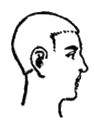
\includegraphics[width=.15\textwidth]{left.jpg}};
      \node[visible on=<1->] (right) [right=4cm  of left] {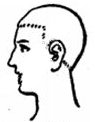
\includegraphics[width=.1\textwidth]{right.jpg}};
      \node[visible on=<2->] (G1) [draw,above=.25cm of left] {Grammar $n$};
      \path[->] (left)  edge[dashed, out=-35,in=215, visible on=<3->] node[below]  {Data $n$} (right);
      \node[visible on=<4->] (G2) [draw,above=.25cm of right] {Grammar $n+1$};
    \end{tikzpicture}
  \end{center}
\end{frame}


\begin{frame}
  \frametitle{Language change}
  \begin{center}
    \begin{tikzpicture}[->,>=stealth',shorten >=1pt,auto,node distance=3cm]
      \node (A)      {Grammar $n$};
      \node (B) [below right of=A]  {Data $n$};
      \node (C) [above right of=B] {Grammar $n+1$};
      \node (D) [below right of=C] {Data $n+1$};
      \node (E) [above right of=D] {};
      \path[->] (A)  edge node[sloped, anchor=center, below] {} (B)
      (B) edge node[sloped, anchor=center, below] {\only<2>{Acquisition}} (C)
      (C) edge[dashed] node {} (D)
      (D) edge[dashed] node {} (E);
    \end{tikzpicture}
  \end{center}
\end{frame}


\begin{frame}{Language change}
  \begin{center}
    \begin{tikzpicture}
      \node[visible on=<1->] (left)      {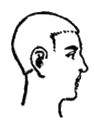
\includegraphics[width=.15\textwidth]{left.jpg}};
      \node[visible on=<1->] (right) [right=4cm  of left] {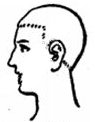
\includegraphics[width=.15\textwidth]{right.jpg}};
      \node[visible on=<2->] (G1) [draw,above=.25cm of left] {Grammar $n$};
      \node[visible on=<2->] (G2) [draw,above=.25cm of right] {Grammar $n$};
      \path[->] (left)  edge[dashed, out=-35,in=220, visible on=<3->] node[below]  {Data $n$} (right);
      \path[->] (right)  edge[dashed, out=215,in=-40, visible on=<3->] (left);
    \end{tikzpicture}
  \end{center}
\end{frame}


\begin{frame}
  \frametitle{Language change}
  \begin{center}
    \begin{tikzpicture}[->,>=stealth',shorten >=1pt,auto,node distance=3cm]
      \node (A)      {Grammar $n$};
      \node (B) [below right of=A]  {Data $n$};
      \node (C) [above right of=B] {Grammar $n+1$};
      \node (D) [below right of=C] {Data $n+1$};
      \node (E) [above right of=D] {};
      \path[->] (A)  edge node[sloped, anchor=center, below] {\only<2>{Use}} (B)
      (B) edge node[sloped, anchor=center, below] {Acquisition} (C)
      (C) edge[dashed] node {} (D)
      (D) edge[dashed] node {} (E);
    \end{tikzpicture}
  \end{center}
\end{frame}

\begin{frame}
\frametitle{Kinds of competence}
\begin{columns}[T]  
   \begin{column}{.2\textwidth}
     % \begin{center}
	  \vspace{20pt}
	  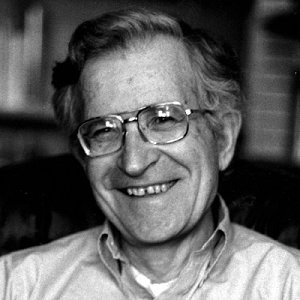
\includegraphics[height=1in]{chomsky.jpg}   
     % \end{center}
   \end{column}
   \begin{column}{.75\textwidth}
      \begin{block}{}
      \begin{quote}
	   By \textbf{grammatical competence} I  mean the cognitive state that encompasses all those aspects of form and meaning and their relation...\textbf{Pragmatic competence} underlies the ability to use such knowledge along with the conceptual system to achieve certain ends or purposes. 
      \end{quote}           
      \end{block}
    \end{column}
  \end{columns}
  \vfill \hfill \citep{chomsky1980rules}
\end{frame}


\begin{frame}
\frametitle{Kinds of competence}
\begin{columns}[T]  
   \begin{column}{.2\textwidth}
     % \begin{center}
	  \vspace{20pt}
	  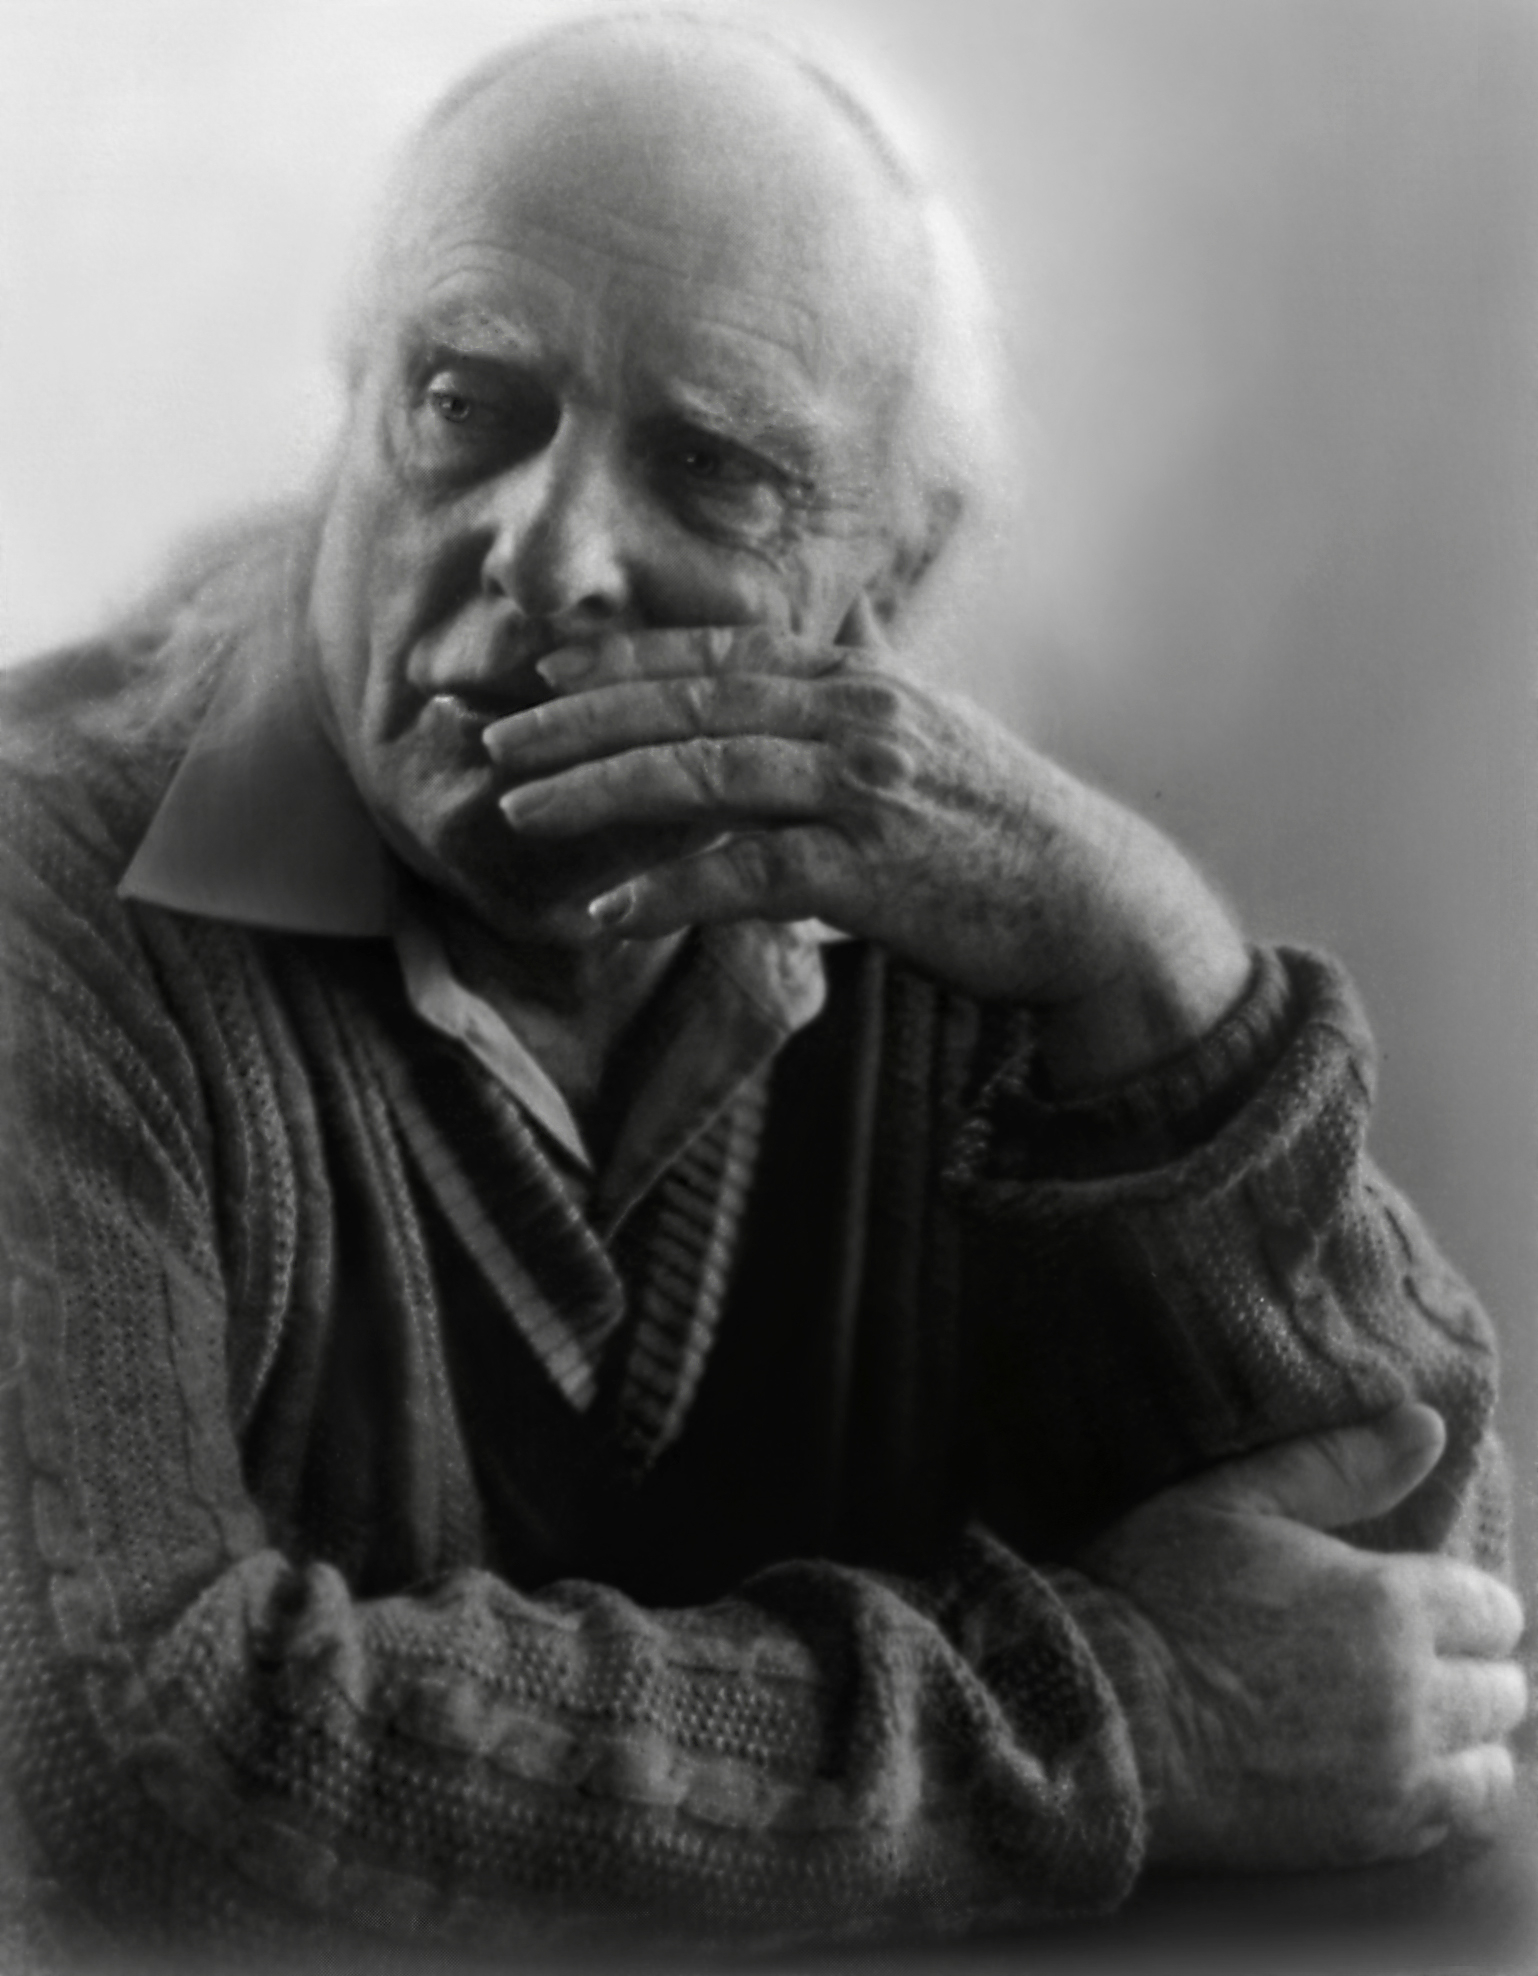
\includegraphics[height=1.2in]{grice.jpg}   
     % \end{center}
   \end{column}
   \begin{column}{.75\textwidth}
      \begin{block}{}
      \begin{quote}
	   I am, however, enough of a \textbf{rationalist} to want to find a basis that underlies these facts, undeniable though they may be; I would like to be able to think of the standard type of conversational practice not merely as something that all or most do \textbf{in fact} follow but as something that it is \textbf{reasonable} for us to follow, that \textbf{we should not abandon}. 
      \end{quote}           
      \end{block}
    \end{column}
  \end{columns}
\vfill \hfill \citep{grice1975}
\end{frame}


\begin{frame}
\frametitle{Kinds of competence}
\only<2>{\emph{Something we might \textbf{reasonably abandon}} (cf. \cite{grice1975}) }
\begin{columns}[T]  
   \begin{column}{.2\textwidth}
     % \begin{center}
	  \vspace{20pt}
	  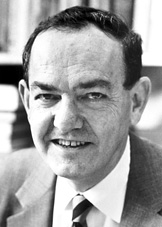
\includegraphics[height=1.2in]{simon.jpg}   
     % \end{center}
   \end{column}
   \begin{column}{.75\textwidth}
      \begin{block}{}
      \begin{quote}
	   The principle of \textbf{bounded rationality}, the capacity of the human mind for formulating and solving complex problems is very small compared with the size of the problems whose solution is required for objectively rational behavior in the real world --- or even for a reasonable approximation to such objective rationality. 
      \end{quote}           
      \end{block}
    \end{column}
  \end{columns}
\vfill \hfill  \citep{simon1947}
\end{frame}


\begin{frame}
\frametitle{Kinds of competence}
	\begin{center}
	  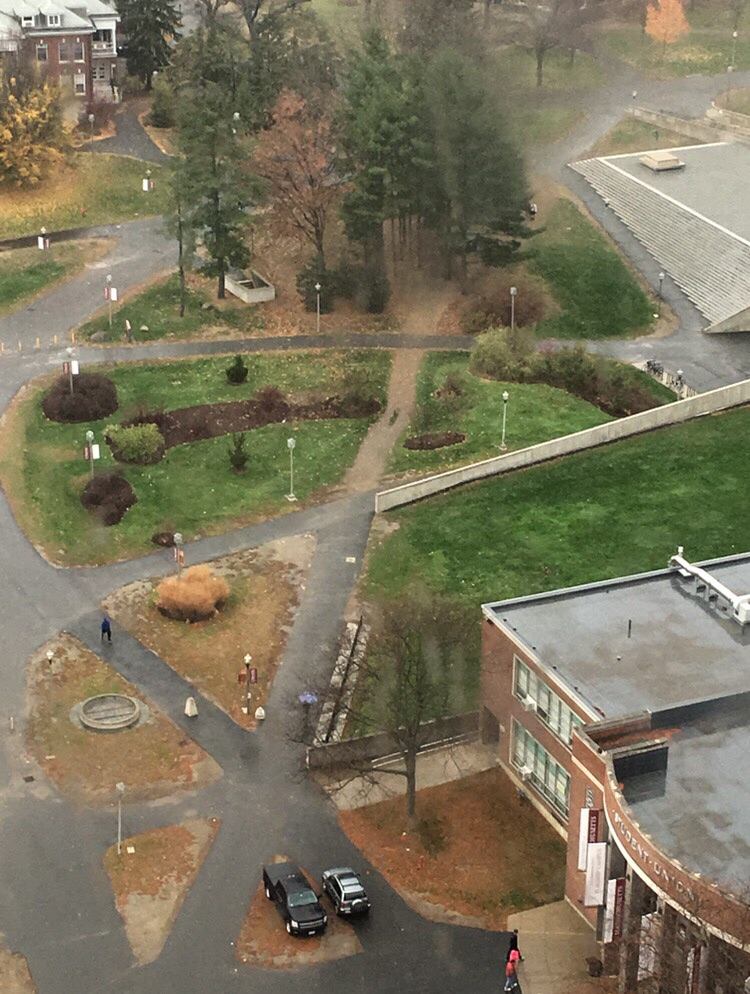
\includegraphics[height=2in]{keller.jpg}   
	 \end{center}
\vfill \hfill (cf. \href{http://i.imgur.com/PAQb1ith.jpg}{reddit.com/r/desirepath}; \cite{Keller:1994})

%http://i.imgur.com/PAQb1ith.jpg
\end{frame}

\begin{frame}
  \frametitle{Kinds of competence}
  \begin{center}
    \begin{tikzpicture}[->,>=stealth',shorten >=1pt,auto,node distance=3cm]
      \node (A)      {Grammar $n$};
      \node (B) [below right of=A]  {Data $n$};
      \node (C) [above right of=B] {Grammar $n+1$};
      \node (D) [below right of=C] {Data $n+1$};
      \node (E) [above right of=D] {};
      \path[->] (A)  edge node[sloped, anchor=center, below] {Use} (B)
      (B) edge node[sloped, anchor=center, below] {Acquisition} (C)
      (C) edge[dashed] node {} (D)
      (D) edge[dashed] node {} (E);
    \end{tikzpicture}
  \end{center}
\end{frame}


\section{Jespersen's cycles}

\begin{frame}
\frametitle{Jespersen's cycle}
\begin{columns}[T]  
   \begin{column}{.2\textwidth}
     % \begin{center}
  	  \vspace{20pt}
	  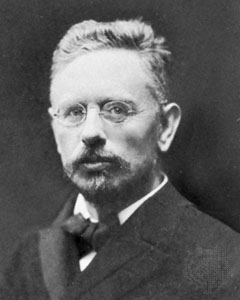
\includegraphics[height=1.2in]{jespersen.jpg}   
     % \end{center}
   \end{column}
   \begin{column}{.75\textwidth}
      \begin{block}{}
      \begin{quote}
      The history of \textbf{negative expressions} in various languages makes us witness the following curious fluctuation: the original negative adverb is first \textbf{weakened}, then found insufficient and therefore \textbf{strengthened}, generally through some additional word, and this in its turn may be felt as the negative proper and may then in course of time be subject to the same developments as the original word.
      \end{quote}
	\end{block}
    \end{column}
  \end{columns}
 \vfill\hfill \citep{jespersen:1917}
\end{frame}


\begin{frame}
  \frametitle{Jespersen's cycle}
  \begin{center}
    \begin{tikzpicture}[->,>=stealth',shorten >=1pt,auto,node distance=3cm]
      \node[draw,circle] (A)      {1};
      \node[draw,circle] (B) [right of=A]  {2};
      \node[draw,circle] (C) [right of=B] {3};
      \node[draw,circle] (D) [right of=C] {4};
      \node[visible on=<2->] (S1) [below=.5cm of A] {\textsc{\textcolor{red}{neg V}}};
      \node[visible on=<3->] (S2) [below=.5cm of B] {\textsc{\textcolor{red}{neg V} \textcolor{blue}{(neg)}}};
      \node[visible on=<4->] (E) [below=.2cm of S2] {\textcolor{blue}{(Emphatic)}};
      \node[visible on=<5->] (S3) [below=.5cm of C] {\textsc{\color{blue} neg V neg}};
      \node[visible on=<6->] (S4) [below=.5cm of D] {\textsc{\color{green} V neg}};
    \end{tikzpicture}
  \end{center}
  
\vfill \hfill \footnotesize{(cf. \citealt{posner1985,schwegler1988,ladusaw1993}, \emph{inter alia})}
\end{frame}

\begin{frame}
\resizebox{\linewidth}{!}{% 
     \begin{tikzpicture}
%draw horizontal line
\draw (0,0) -- (16,0);
%draw ticks
\foreach \x in {0, 2, 4, 6, 8, 10, 12, 14, 16}{
   \draw (\x,3pt) -- (\x,-3pt);
}
%draw tick dates
\draw (0,0) node[below=3pt] { 400 } node[above=10pt] { };
\draw (4,0) node[below=3pt] { 800 } node[above=10pt] { };
\draw (8,0) node[below=3pt, visible on=<1-14>] { 1200 } node[above=3pt] { };
\draw (12,0) node[below=3pt] { 1600 } node[above=3pt] { };
\draw (16,0) node[below=3pt] { 2000 } node[above=3pt] {  };
% draw nodes and pictures for historical context
% \draw (0,0) node[below=1.5in, anchor=south west, visible on=<2->] { 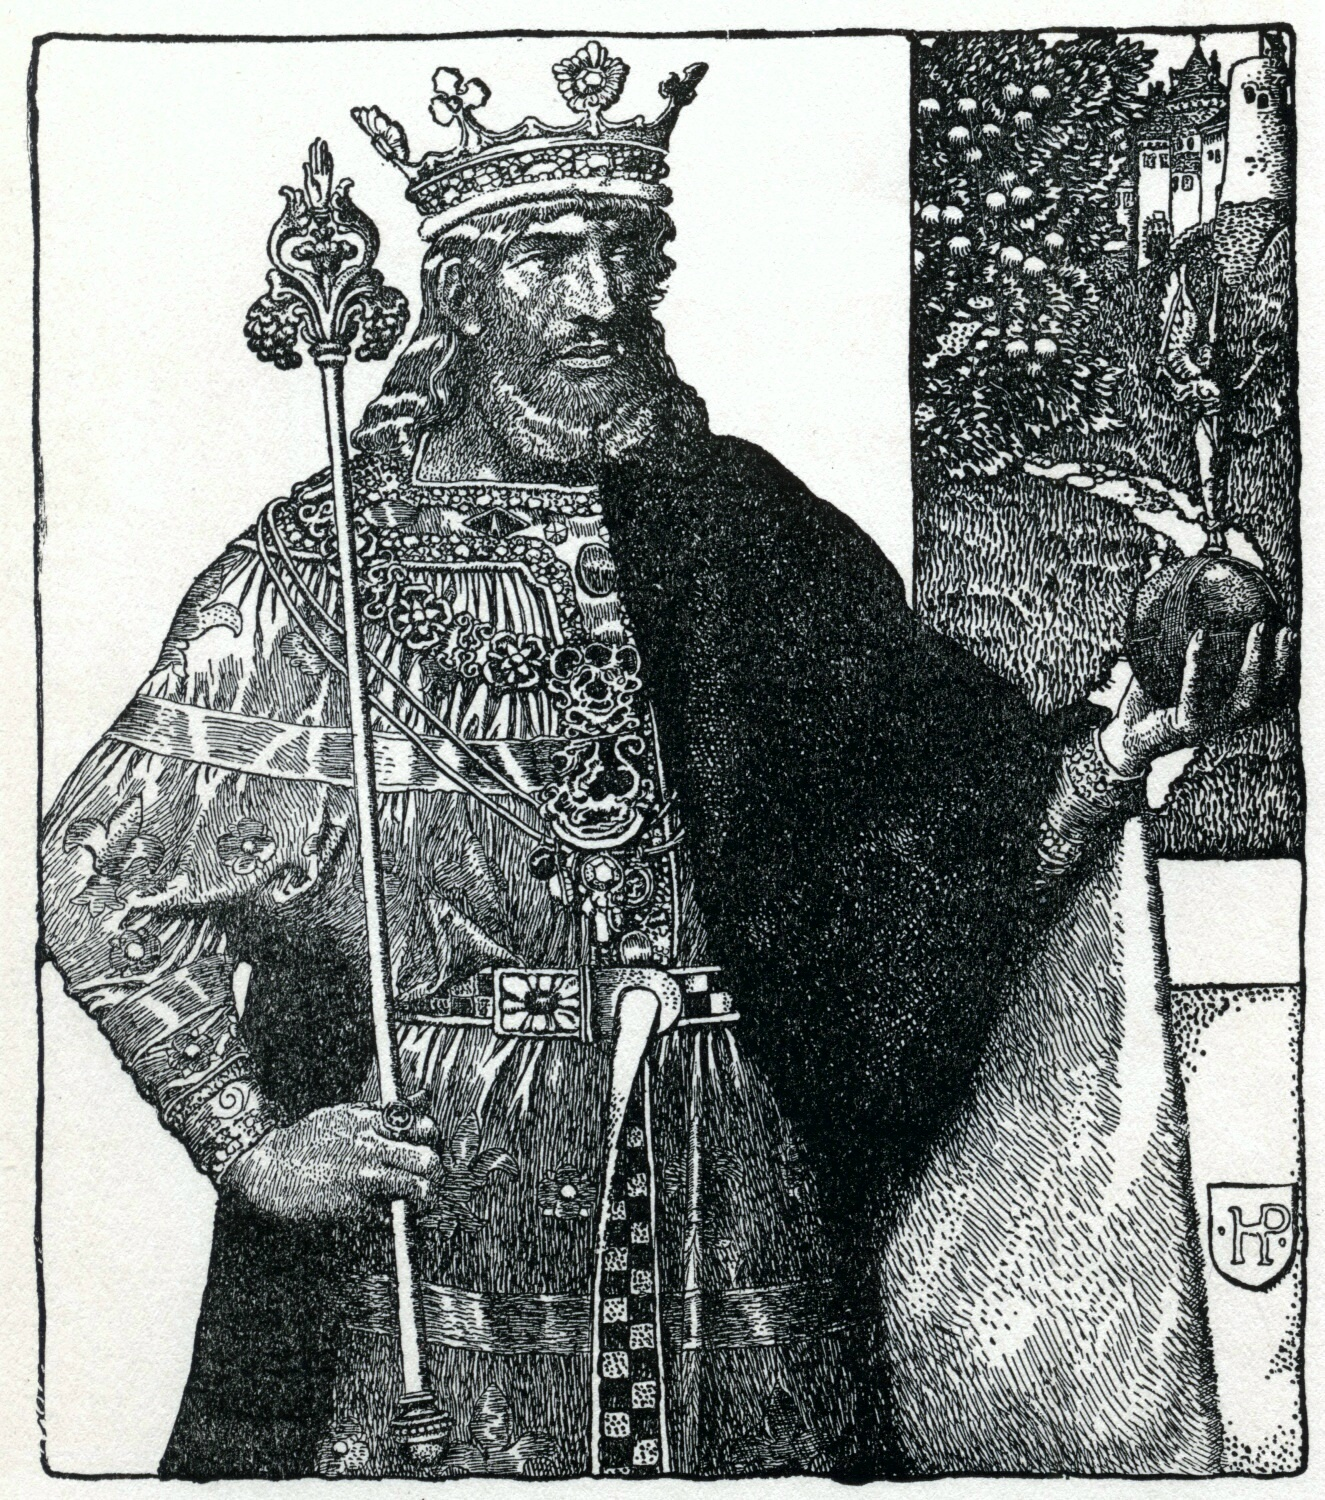
\includegraphics[width=.2\textwidth]{arthur.jpg} };
\draw (4,0) node[below=2in, anchor=south west, visible on=<2->] { 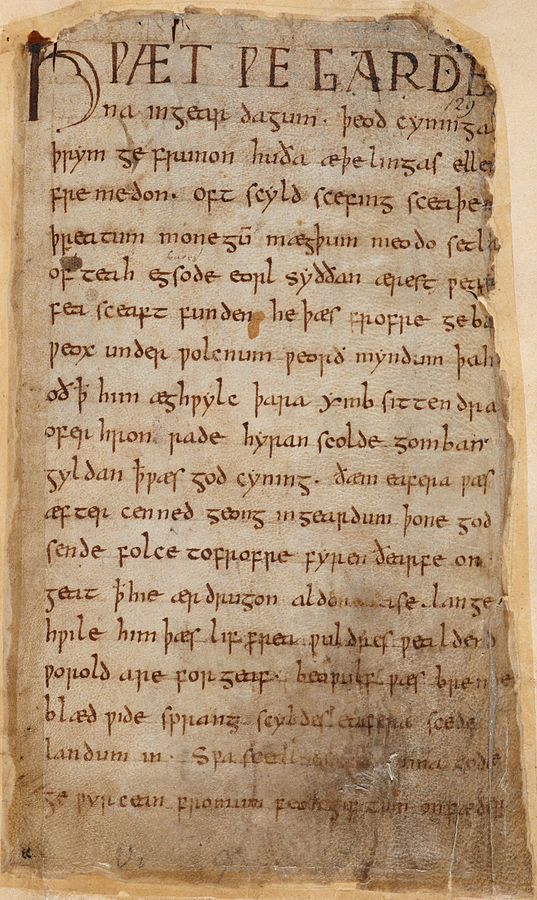
\includegraphics[width=.2\textwidth]{beowulf.jpg} };
\draw (7.5,0) node[below=1.65in, anchor=south west, visible on=<3->] { 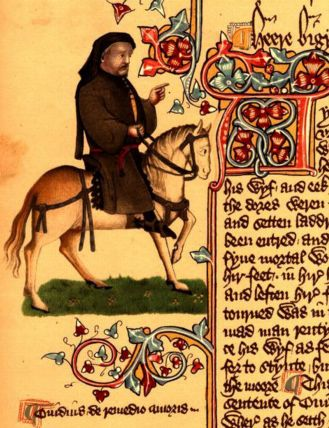
\includegraphics[width=.2\textwidth]{chaucer.jpg} };
\draw (11,0) node[below=1.65in, anchor=south west, visible on=<4->] { 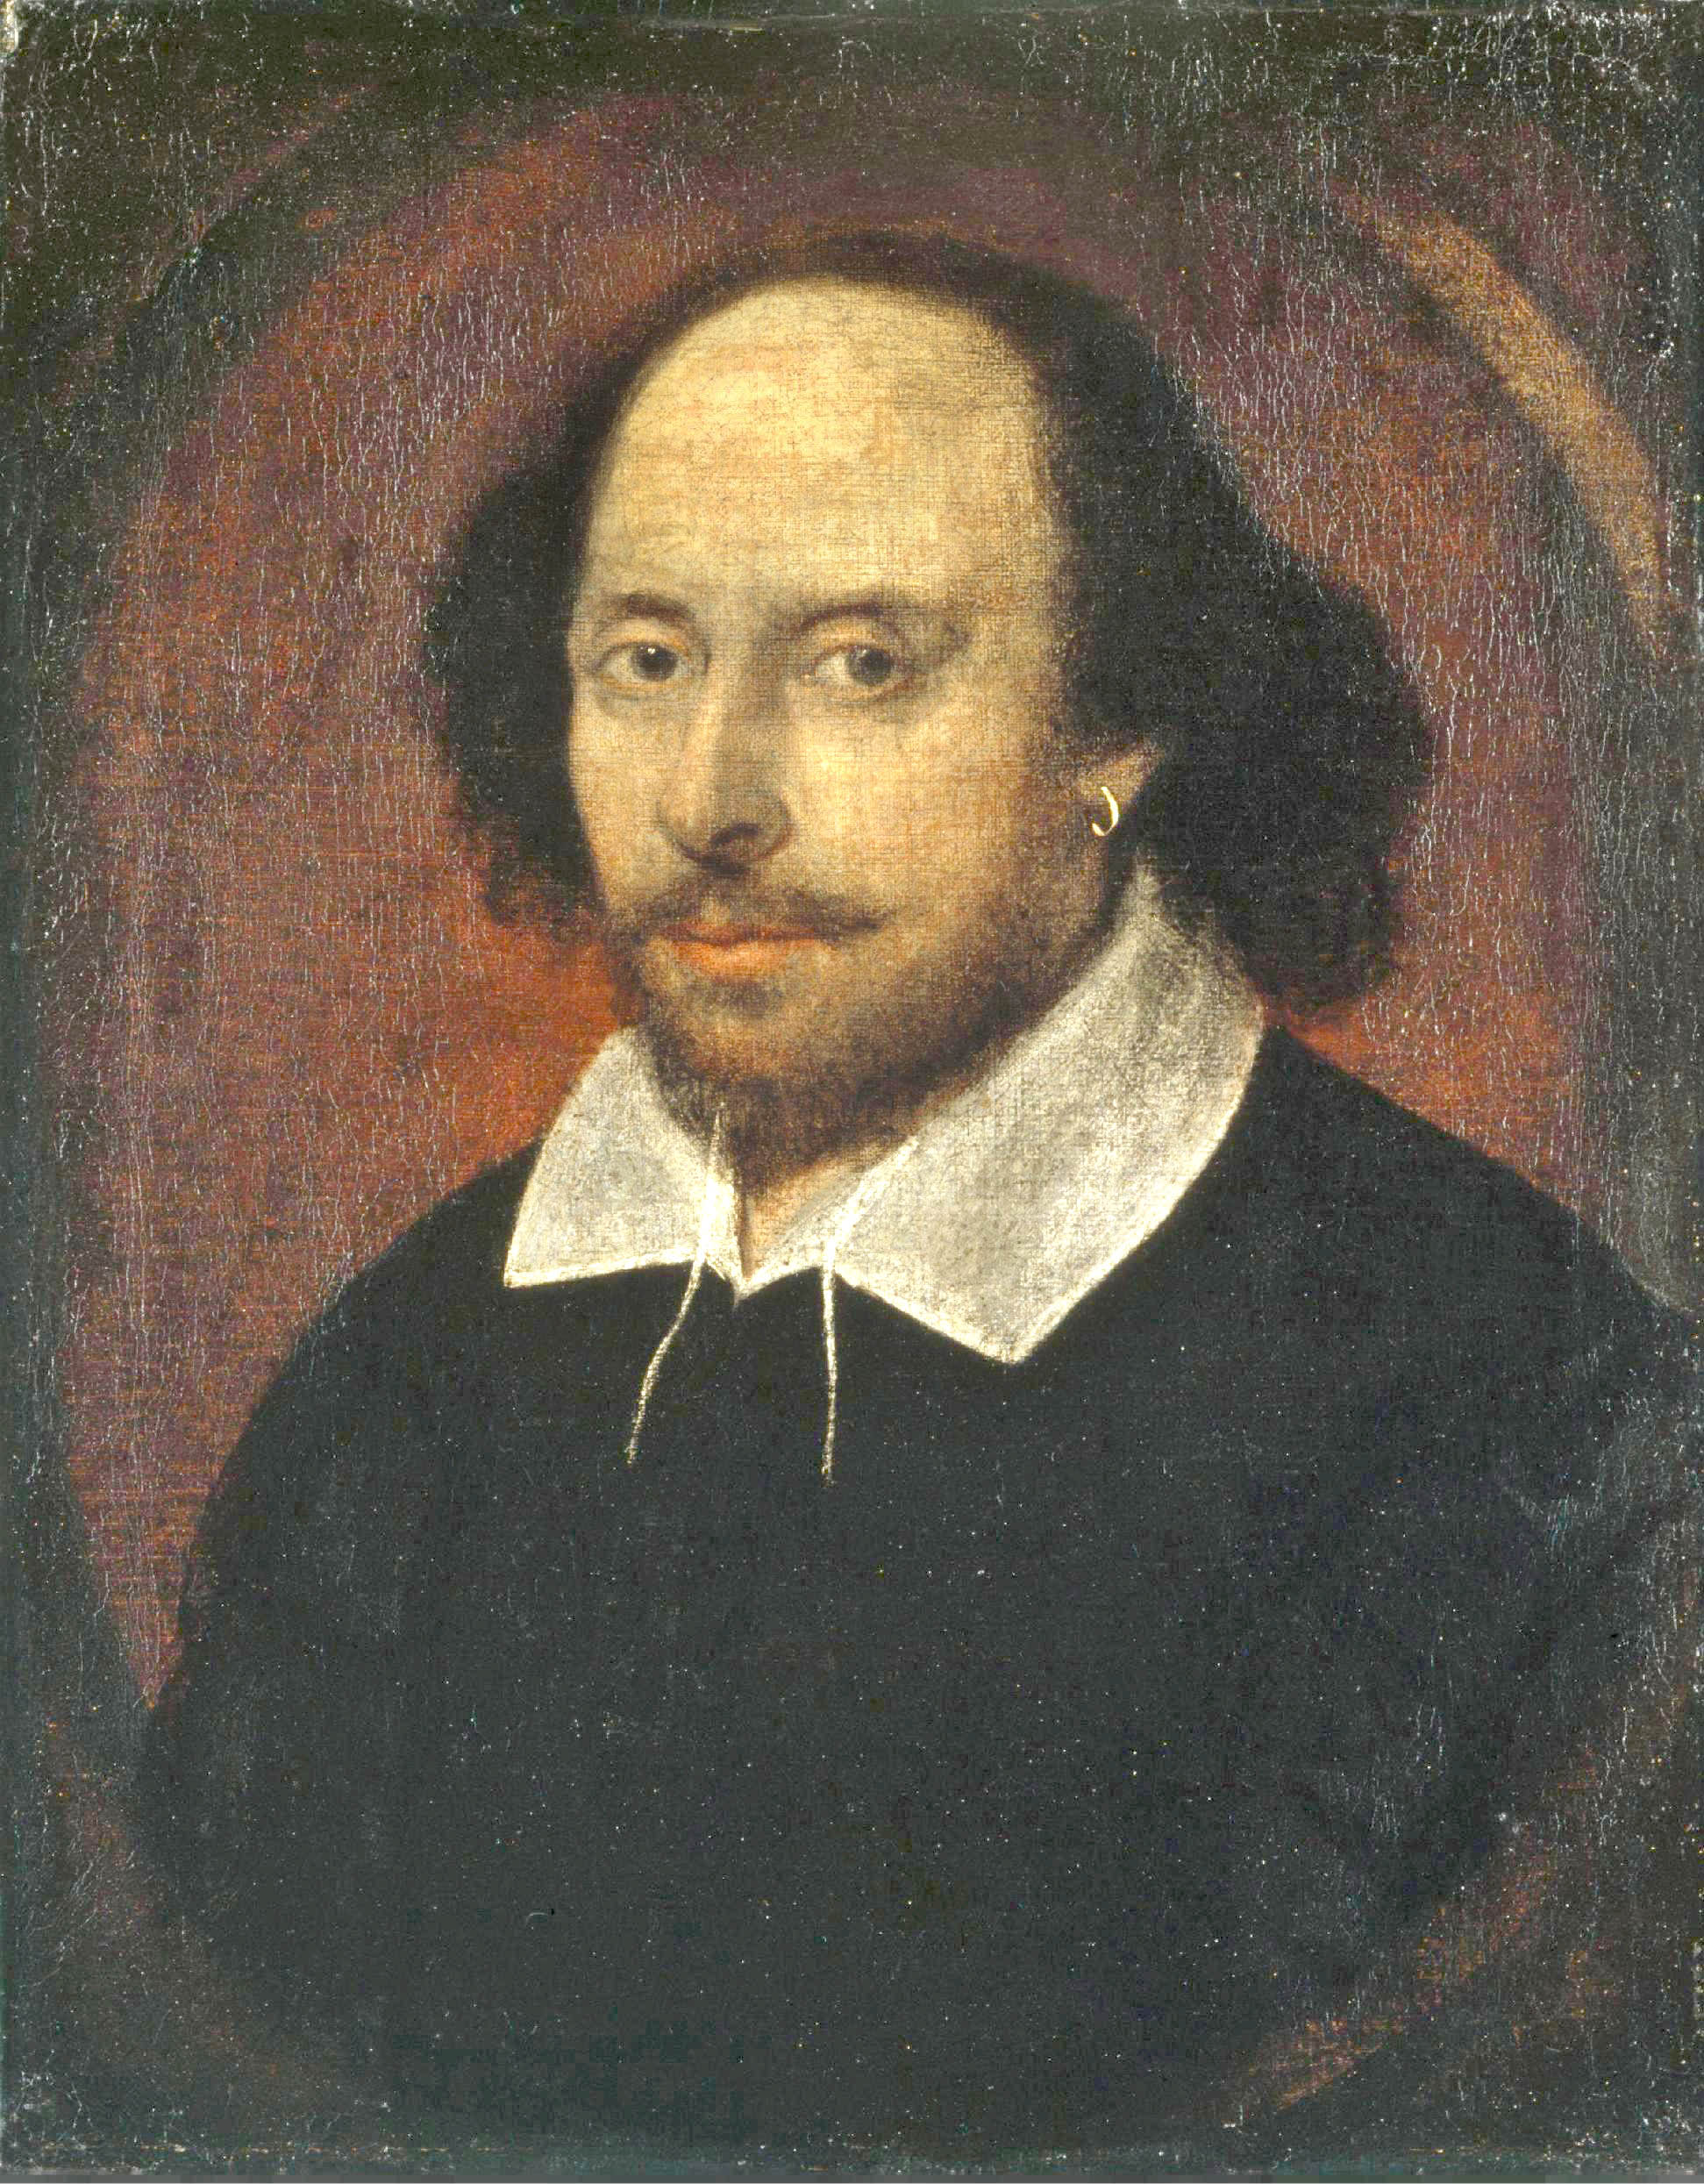
\includegraphics[width=.2\textwidth]{shakespeare.jpg} };
\draw (15,-2.5) node[visible on=<5->] {$\dots$};
% Add 
\draw [ultra thick, visible on=<6-14>] (0,.5) to (7.4,.5);
\draw (3.75, 1) node[visible on=<6-14>] {Old English};
\draw [ultra thick, visible on=<7-14>] (7.5,.5) to (10.4,.5);
\draw (9, 1) node[visible on=<7->] {Middle English};
\draw [ultra thick, visible on=<8-14>] (10.5,.5) to (12.4,.5);
\draw (11.5, 1) node[text width=2cm,align=center, visible on=<8-14>] {E. Modern English};
\draw [ultra thick, visible on=<9-14>] (12.5,.5) to (16,.5);
\draw (14.25, 1) node[visible on=<9-14>] {Modern English};
% draw ticks for historical examples
% ne 		: 400-1300
% ne..not	: 1100-1400
% not		: 1350-1700
% do not 	: 1500-2000
\draw [ultra thick,red, visible on=<10->] (2,2) to (10,2);
\draw (3.75, 2.5) node[red, visible on=<10->] {Ic ne secge};
\draw [ultra thick,blue, visible on=<11->] (7,2.25) to (11,2.25);
\draw (8.5, 2.75) node[blue,visible on=<11->] {I ne seye not};
\draw [ultra thick,green, visible on=<12->] (9.75,2.5) to (13,2.5);
\draw (10.75, 3) node[green, visible on=<12->] {I say not};
\draw [ultra thick, red, visible on=<13->] (11.75,2.75) to (16,2.75);
\draw (14, 3.25) node[red, visible on=<13->] {I do not say};
% draw negative forms
\draw (3.75,4) node [above,visible on=<14->] {\textsc{\color{red} neg V}};
\draw (8.5,4) node [above,visible on=<14->] {\textsc{\color{blue} neg V neg}};
\draw (10.75,4) node [above,visible on=<14->] {\textsc{\color{green} V neg}};
\draw (14,4) node [above,visible on=<14->] {\textsc{\color{red} neg V}};
\draw [ultra thick,visible on=<15->] (6.5,-.75) -- (11.5,-.75) -- (11.5,3.5) -- (6.5,3.5) -- (6.5,-.75);
\draw (7,0) node[below=3pt, visible on=<15->] {1100 };
\draw [ultra thick,visible on=<15->] (7,3pt) -- (7,-3pt);
\draw (11,0) node[below=3pt, visible on=<15->] { 1500 };
\draw [ultra thick,visible on=<15->] (11,3pt) -- (11,-3pt);
\draw [ultra thick,visible on=<15->] (7,0) -- (11,0);
\draw [ultra thick,visible on=<16->] (2.75,3.75) -- (11.75,3.75) -- (11.75,5) -- (2.75,5) -- (2.75,3.75);
\draw (11,5) node [above,visible on=<17->] {The formal cycle};
\draw [ultra thick,visible on=<18->] (3,4) -- (9.75,4) -- (9.75,4.75) -- (3,4.75) -- (3,4);
\draw (3.5,5) node [above,visible on=<19->] {The functional cycle};
\end{tikzpicture}
}
\end{frame}



\begin{frame}
	\frametitle{The formal cycle}
	\begin{center}
\begin{tikzpicture}
	% Define margin to offset
	\def \margin {8}
	% Draw nodes
	\node[draw,circle] at ({90}:3) {2};
	\node[draw,circle] at ({270}:3) {1};
	% Draw arcs
	\draw[->, >=latex] ({270 - \margin}:3) arc ({270 - \margin}:{90 + \margin}:3);
	\draw[->, >=latex] ({90 - \margin}:3) arc ({90 - \margin}:{-90 + \margin}:3);
	% Draw complexity axis
	\draw[->, >=latex] (-5,-3) -- (-5,3);
	\node[align=center,text width=2cm] at (-6.25, 0) {Formal complexity};
\end{tikzpicture}
	\end{center}
\end{frame}


\begin{frame}
\frametitle{The formal cycle}
	\begin{center}
\begin{tikzpicture}[->,>=stealth',shorten >=1pt,auto,node distance=3cm]
  \node (A)      {\textsc{\textcolor{red}{neg V}}};
  \node (B) [above right of=A]  {\textsc{\color{blue} neg V neg}};
  \node (C) [below right of=B] {\textsc{\color{green} V neg}};
  \node (D) [left of=A] {};
  \node (E) [above of=D] {};
\path[->] (A)  edge node {} (B)
  (B) edge node {} (C);
	% Draw axes
    \draw[->] (-1.5,0) -- (-1.5,2);
  \node[align=center, text width=2cm] at (-2.75, 1) {Formal complexity};
    \draw[->] (0,-1) -- (4,-1);
    \node at (2,-1.5) {Time};
\end{tikzpicture}
	\end{center}
\end{frame}


\begin{frame}
\frametitle{The formal cycle}
\textbf{Doesn't} require return to pre-verbal negation:
\begin{center}

\ex. I do \textcolor{red}{not} say\\

\ex. I do\textcolor{red}{n't} say\\

\vfill \hfill (EME: \cite{ellegaard1953})
\end{center}
\end{frame}


\begin{frame}
\frametitle{The formal cycle}
\textbf{Doesn't} require post-verbal element for increased complexity:
\begin{center}

\ex. You do\textcolor{blue}{n't eem} know.

\ex. You \textcolor{red}{eem} know.

\vfill \hfill (AAVE: \cite{jones2015})
\end{center}
%\cite{jones2015}
\end{frame}


\begin{frame}
	\frametitle{The functional cycle}
	\begin{center}
\begin{tikzpicture}
	% Define margin to offset
	\def \margin {8}
	% Draw nodes
	\node[draw,circle] at ({90}:3) {2};
	\node[draw,circle] at ({270}:3) {1};
	% Draw arcs
	\draw[->, >=latex] ({270 - \margin}:3) arc ({270 - \margin}:{90 + \margin}:3);
	\draw[->, >=latex] ({90 - \margin}:3) arc ({90 - \margin}:{-90 + \margin}:3);
	% Draw complexity axis
	\draw[->, >=latex] (-5,-3) -- (-5,3);
	\node[align=center,text width=3cm] at (-6.75, 0) {Functional distinctions};
\end{tikzpicture}
	\end{center}
\end{frame}

\begin{frame}
\frametitle{The functional cycle}
\begin{columns}[T]  
   \begin{column}{.2\textwidth}
     % \begin{center}
  	  \vspace{12pt}
	  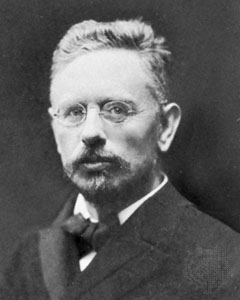
\includegraphics[height=1.2in]{jespersen.jpg}   
     % \end{center}
   \end{column}
   \begin{column}{.75\textwidth}
      \begin{block}{}
      \begin{quote}
	But in most cases the addition serves to make the negative more impressive as being \textbf{more vivid or picturesque}, generally through an \textbf{exaggeration}, as when substantives meaning something very small are used as subjuncts.
      \end{quote}
	\end{block}
    \end{column}
  \end{columns}
 \vfill\hfill \citep{jespersen:1917}
\end{frame}

\begin{frame}
\frametitle{The functional cycle}
Could have been called \emph{Meillet's spiral} \citep{vanderAuwera2009}:
\begin{columns}[T]  
   \begin{column}{.2\textwidth}
     % \begin{center}
  	  \vspace{12pt}
	  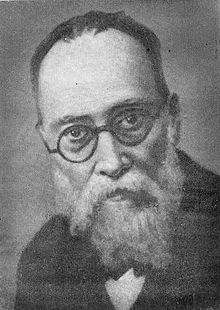
\includegraphics[height=1.2in]{meillet.jpg}   
     % \end{center}
   \end{column}
   \begin{column}{.8\textwidth}
      \begin{block}{}
\begin{quote}
Thus, languages follow a sort of spiral development: they \textbf{add extra words to intensify expression}; these words fade; decay and fall to the level of simple grammatical tools; \textbf{one adds new or different words} on account of expressiveness; the fading begins again, and so on endlessly.
\end{quote}
	\end{block}
    \end{column}
  \end{columns}
 \vfill\hfill \citep{meillet1912}\\
 \only<2>{\hfill or \emph{Gardiner's gyre} \citeyearpar{gardiner1904}}
\end{frame}


\begin{frame}
	\frametitle{The functional cycle}
\begin{center}
\begin{tikzpicture}[->,>=stealth',shorten >=1pt,auto,node distance=3cm]
  \node[draw,circle] (A)      {1};
  \node[draw,circle] (B) [above right of=A]  {2};
  \node[draw,circle] (C) [below right of=B] {2};
  \node[draw,circle] (D) [below right of=A] {1};
\path[->] (A)  edge node {} (D)
  (B) edge node {} (C);
	% Draw axes
    \draw[->] (-1.5,-2.5) -- (-1.5,2.5);
  \node[align=center, text width=2cm] at (-2.75, 0) {Emphasis};
    \draw[->] (0,-3) -- (4,-3);
    \node at (2,-3.5) {Time};
\end{tikzpicture}
\end{center}
\end{frame}


\begin{frame}
	\frametitle{The functional cycle}
\begin{center}
\begin{tikzpicture}[->,>=stealth',shorten >=1pt,auto,node distance=3cm]
  \node (A)      {\textsc{\textcolor{red}{neg V}}};
  \node (B) [above right of=A]  {\textsc{\color{blue} neg V neg}};
  \node (C) [below right of=B] {\textsc{\color{blue} neg V neg}};
  \node (D) [below right of=A] {\textsc{\textcolor{red}{neg V}}};
\path[->] (A)  edge node {} (D)
  (B) edge node {} (C);
	% Draw axes
    \draw[->] (-1.5,-2.5) -- (-1.5,2.5);
  \node[align=center, text width=2cm] at (-2.75, 0) {Emphasis};
    \draw[->] (0,-3) -- (4,-3);
    \node at (2,-3.5) {Time};
\end{tikzpicture}
\end{center}
\end{frame}


\begin{frame}{The functional cycle}
\textbf{Doesn't} coincide with the formal cycle:

\begin{center}
	\textsc{\textcolor{red}{neg V }} $\subset$ \textsc{\textcolor{blue}{neg V neg}} $\not\subset$ \textsc{\textcolor{green}{ V neg}}
\end{center}
      \vfill\hfill \citep{frege1884}
\end{frame}


\begin{frame}{The functional cycle}
\textbf{Doesn't} require a formal cycle:

  \begin{table}[ht]
    %\begin{center}
    \begin{tabular}{@{}ccc@{}}
      \hline
      \textsc{plain} & \textsc{emphatic} & \textsc{source} \\
      \hline
      \textgreek{ou...ti} & \textgreek{ou-de...en} & Ancient Greek \\
      \textgreek{(ou)den...ti} & \only<1,3->{\textgreek{den...tipote}} \only<2>{\textcolor{blue}{\textgreek{den...tipote}}} & Early Medieval Greek \\
       \only<1,3->{\textgreek{den...tipote}} \only<2>{\textcolor{blue}{\textgreek{den...tipote}}} & \only<1-2,4->{\textgreek{den... prama}} \only<3>{\textcolor{blue}{\textgreek{den... prama}}} & Greek Dialects \\
      \only<1-2,4->{\textgreek{den... prama}} \only<3>{\textcolor{blue}{\textgreek{den... prama}}} & \textgreek{den...apantoxh} & Modern Cretan \\
      \hline
    \end{tabular}
    %\end{center}
  \end{table}
   \only<2->{\hfill \emph{One adds \textbf{new or different} words} \citep{meillet1912}}
      \vfill\hfill \citep{kiparsky-condoravdi:2006}
\end{frame}


\begin{frame}
	\begin{center}
\begin{tikzpicture}[node distance=3cm]
  \node (A)      {\color{red} \textsc{neg V}};
  \node (B) [right of=A]  {\color{blue} \textsc{neg V neg}};
  \node (C) [right of=B] {\color{green} \textsc{V neg}};
  \draw [ultra thick, visible on=<2->] (-1,-1) -- (7,-1) -- (7,1) -- (-1,1) -- (-1,-1);
  \draw (6,1.25) node [above,visible on=<3->] {The formal cycle};
%  \draw [ultra thick,visible on=<4->] (-.75,-.75) -- (4.25,-.75) -- (4.25,.75) -- (-.75,.75) -- (-.75,-.75);
%  \draw (0,1.25) node [above,visible on=<5->] {The functional cycle};
\end{tikzpicture}
	\end{center}
\end{frame}


\begin{frame}
\frametitle{A pull chain between elements}
%\emph{ne} pulls in \emph{not}:
\begin{columns}[T]  
   \begin{column}{.2\textwidth}
     % \begin{center}
  	  \vspace{12pt}
	  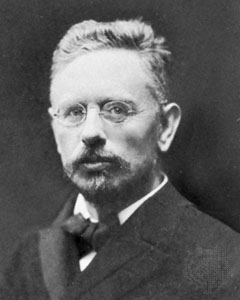
\includegraphics[height=1.2in]{jespersen.jpg}   
     % \end{center}
   \end{column}
   \begin{column}{.8\textwidth}
      \begin{block}{}
      \begin{quote}
The incongruity between the notional importance and the formal insignificance of the negative (often, perhaps, even \textbf{the fear of the hearer failing to perceive it}) may then cause the speaker to \textbf{add something} to make the sense perfectly clear to the hearer.
      \end{quote}
	\end{block}
    \end{column}
  \end{columns}
 \vfill\hfill \citep{jespersen:1917}
\end{frame}


\begin{frame}
\frametitle{ \only<1-2>{A pull chain between elements}\only<3->{\sout{A pull chain between elements}} }
\only<3>{Speakers \textbf{don't} necessarily correct for ambiguity: }
\begin{columns}[T]  
   \begin{column}{.2\textwidth}
     % \begin{center}
  	  \vspace{12pt}
	  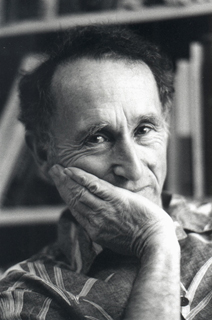
\includegraphics[height=1.2in]{labov.jpg}   
     % \end{center}
   \end{column}
   \begin{column}{.8\textwidth}
      \begin{block}{}
      \begin{quote}
	A very common utterance among residents of this Northern New Jersey area was \textbf{``Did you say C--A--N or C--A--N--T?,''} since the vowel is tense in both words and the /t/ is often neutralized before a following apical obstruent (as in ``I can't tell you'').
      \end{quote}
	\end{block}
    \end{column}
  \end{columns}
 \vfill\hfill \citep{Labov:2010}\\
 \hfill \only<2->{\href{http://www.ispot.tv/ad/7dW0/chevrolet-oil-change-soccer-player}{I can't tell!}}
% http://www.ispot.tv/ad/7dW0/chevrolet-oil-change-soccer-player
%After receiving Chevy certified service, a woman and her soccer-playing son are good to go. After seeing how clean her car is and how dirty her son is, she asks the associate to leave in the paper floor covers. Unfortunately, she can't run him through the car wash.
\end{frame}



\begin{frame}
\frametitle{A push chain between elements}
%\emph{ne} pulls in \emph{not}:
      \begin{block}{}
      \begin{quote}
[T]he reanalyzed construction structurally contains two items which are equally labeled NEG. As a reaction, the ellipsis of \emph{ne} is generalized to all sorts of contexts as well. By way of this process, a \textbf{"simple" function} such as unmarked negation comes to be represented by a morphosyntactically \textbf{"simple" form}. The direction of this change is determined by the principle of \textbf{constructional iconicity}       
	\end{quote}
	\end{block}
 \vfill\hfill (\citealt{detges-waltereit2002}, cf. \citealt{frisch1997})
\end{frame}

\begin{frame}
\frametitle{ \only<1-2>{A push chain between elements}\only<3->{\sout{A push chain between elements}} }
\only<3>{Speakers \textbf{don't} necessarily eliminate redundancy:}
\begin{columns}[T]  
   \begin{column}{.2\textwidth}
     % \begin{center}
%	  \vspace{20pt}
	  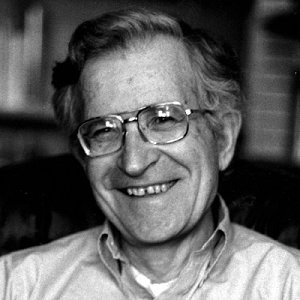
\includegraphics[height=1in]{chomsky.jpg}   
     % \end{center}
   \end{column}
   \begin{column}{.7\textwidth}
      \begin{block}{}
      \begin{quote}
		\only<1>{Colorless green ideas sleep furiously}
		\only<2>{As ideias verdes incolores dormem furiosamente}
		\only<3->{\textbf{As ideias verdes incolores dormem} furiosamente}
      \end{quote}           
      \end{block}
    \end{column}
  \end{columns}
  \vfill \hfill \citep{chomsky1957}
\end{frame}


\begin{frame}
	\begin{center}
\begin{tikzpicture}[node distance=3cm]
  \node (A)      {\color{red} \textsc{neg}};
  \node (B) [right of=A]  {\color{blue} \textsc{neg V neg}};
  \node (C) [right of=B] {\color{green} \textsc{neg}};
%  \draw [ultra thick, visible on=<2->] (-1,-1) -- (7,-1) -- (7,1) -- (-1,1) -- (-1,-1);
%  \draw (6,1.25) node [above,visible on=<3->] {The formal cycle};
  \draw [ultra thick,visible on=<2->] (-.75,-1) -- (4.25,-1) -- (4.25,1) -- (-.75,1) -- (-.75,-1);
  \draw (0,1.25) node [above,visible on=<3->] {The functional cycle};
\end{tikzpicture}
	\end{center}
\end{frame}


\begin{frame}
\frametitle{A push chain between forms}
\only<2>{Depends on what we mean by \textbf{emphatic}:}
      \begin{block}{}
      \begin{quote}
		\textbf{Emphatic negation tends to increase in frequency} due to pragmatically motivated overuse which is characteristic of inherently bounded evaluative scales. This rise in frequency at the expense of plain negation has an \textbf{inflationary effect}, well attested also in politeness systems, hypocoristics, pejoratives, and scalar adjectives of all kinds
	\end{quote}
	\end{block}
 \vfill\hfill (\cite{kiparsky-condoravdi:2006}, cf. \cite{dahl:2001})
\end{frame}



\begin{frame}
\frametitle{The facts to be explained}
	\begin{center}
		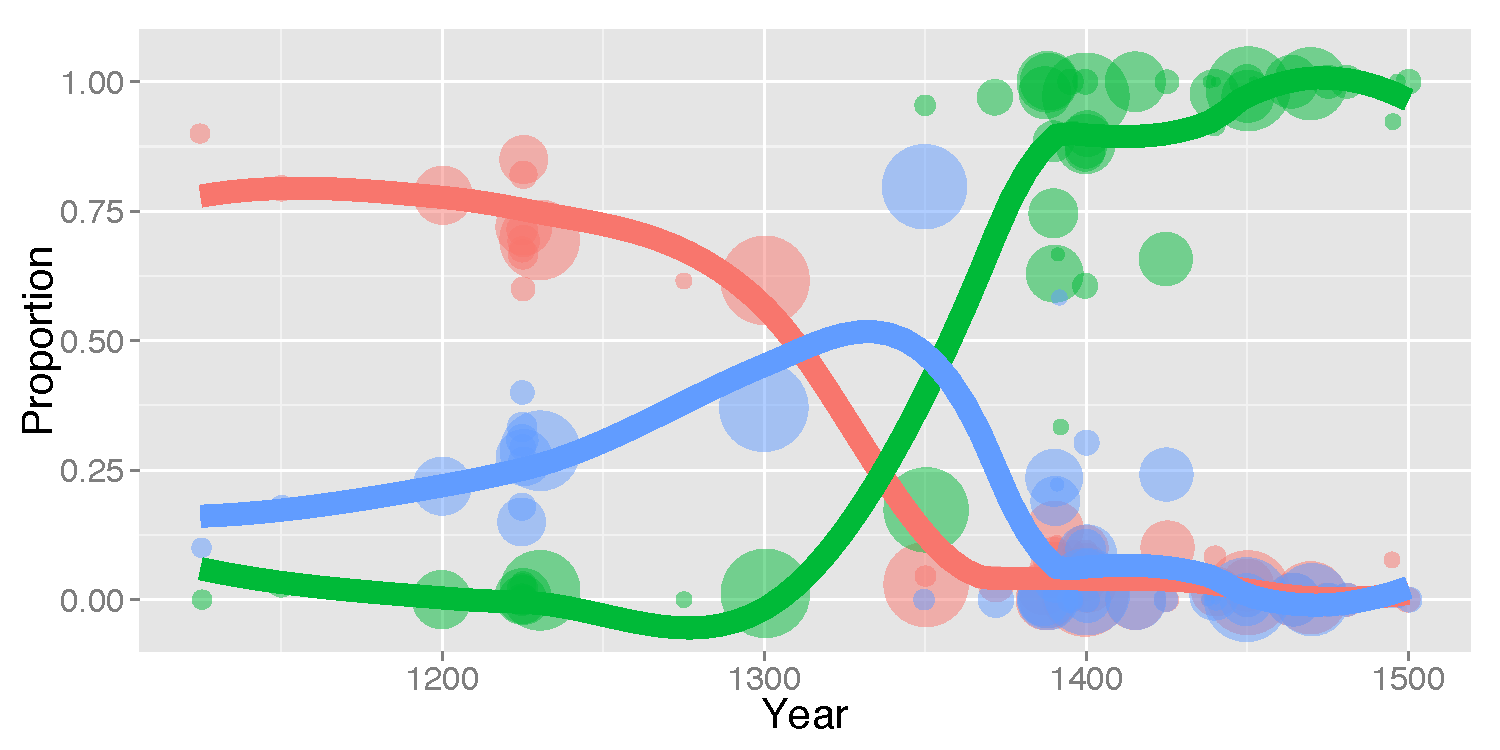
\includegraphics[width=.75\textwidth]{neg-docs-lines.pdf}\\
		\emph{\textcolor{red}{ne}} $\rightarrow$ \emph{\textcolor{blue}{ne...not}} $\rightarrow$ \emph{\textcolor{mygreen}{not}}
	\end{center}
	\vfill \hfill Data from PPCME \citep{ppcme2} 
\end{frame}


\begin{frame}
\frametitle{The role of use in the functional cycle}
  \begin{center}
    \begin{tikzpicture}[->,>=stealth',shorten >=1pt,auto,node distance=3.5cm]
      \node (C)  { \emph{\textcolor{red}{ne} \textcolor{blue}{(...not)}} };
      \node (D) [below right of=C] { \emph{\color{blue} ne...not} };
      \node (E) [above right of=D] {\emph{\color{blue} ne...not} };
      \path[->] (C) edge node[sloped, anchor=center, below] {Use} (D)
      (D) edge node[sloped, anchor=center, below] {} (E);
    \end{tikzpicture}
  \end{center}
\end{frame}


\begin{frame}
\frametitle{The role of acquisition in the formal cycle}
  \begin{center}
  \only<1>{
    \begin{tikzpicture}[->,>=stealth',shorten >=1pt,auto,node distance=3.5cm]
      \node (C)  { \emph{\textcolor{red}{ne} \textcolor{blue}{(...not)}} };
      \node (D) [below right of=C] { \emph{\textcolor{red}{ne} \textcolor{blue}{(...not)}}  };
      \node (E) [above right of=D] {\emph{\color{blue} ne...not} };
      \path[->] (C) edge node[sloped, anchor=center, below] {} (D)
      (D) edge node[sloped, anchor=center, below] {Acquisition} (E);
    \end{tikzpicture}
    }
    \only<2>{
    \begin{tikzpicture}[->,>=stealth',shorten >=1pt,auto,node distance=3.5cm]
      \node (C)  { \emph{\textcolor{blue}{(ne...)} \textcolor{green}{not}} };
      \node (D) [below right of=C] { \emph{\textcolor{blue}{(ne...)} \textcolor{green}{not}}  };
      \node (E) [above right of=D] {\emph{\color{green} not} };
      \path[->] (C) edge node[sloped, anchor=center, below] {} (D)
      (D) edge node[sloped, anchor=center, below] {Acquisition} (E);
    \end{tikzpicture}
    }
  \end{center}
\end{frame}

\begin{frame}
	\frametitle{Main contributions}
	\begin{itemize}
		\item Distinction between formal and functional Jespersen cycles
		\item Model of the dynamics of use in the functional cycle
		\item Model of the dynamics of acquisition in the formal cycle
		\item Application of statistical method for detecting random drift
	\end{itemize}
\end{frame}



%%%%%%%%%%%%%%%%%%%%%%%%%%%%%%%%%%%%%%%%%%%%%%%%%%
\section{The functional cycle}


\begin{frame}
\frametitle{The functional cycle}
	\begin{center}
		\only<1>{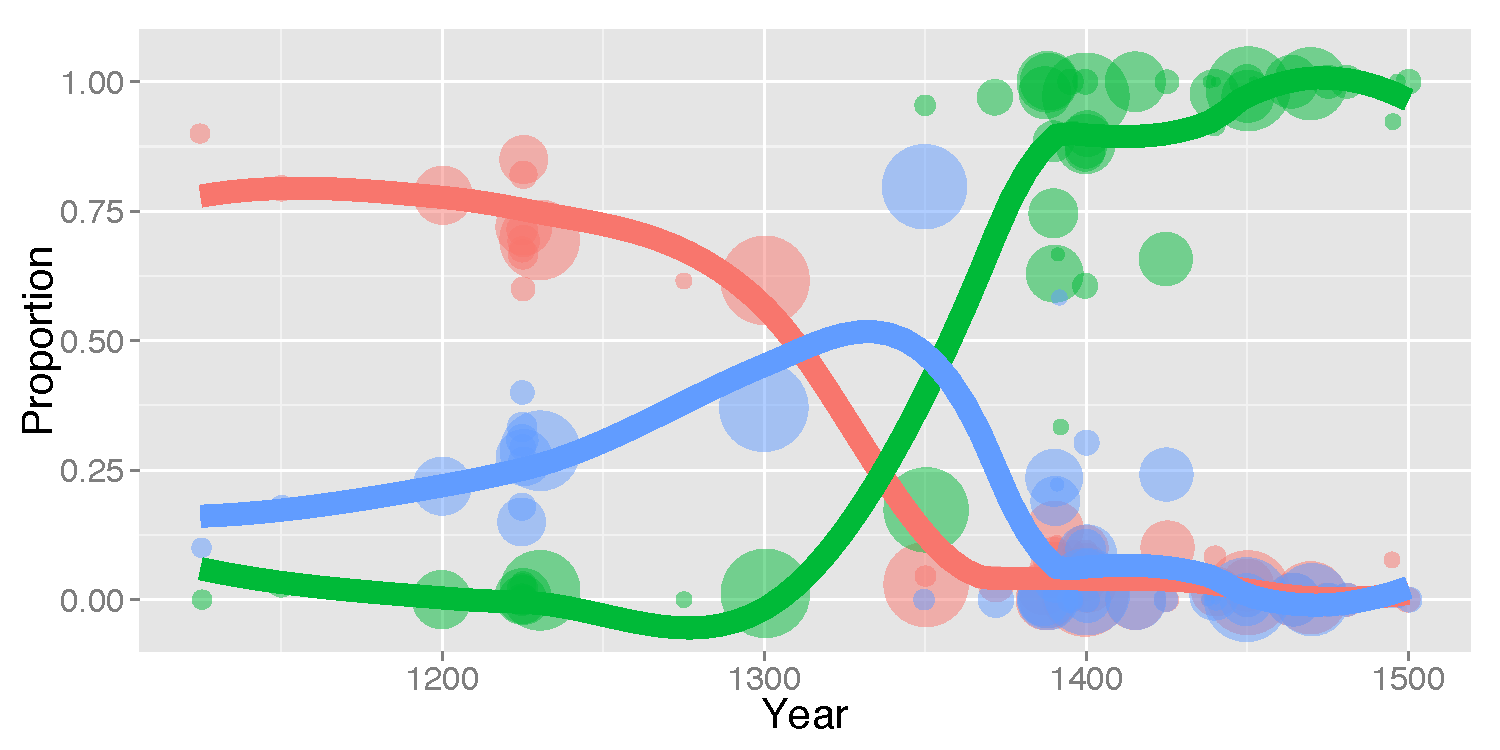
\includegraphics[width=.75\textwidth]{neg-docs-lines.pdf}\\}
		\only<1>{\emph{\textcolor{red}{ne}} $\rightarrow$ \emph{\textcolor{blue}{ne...not}} $\rightarrow$ \emph{\textcolor{mygreen}{not}}}
		\only<2>{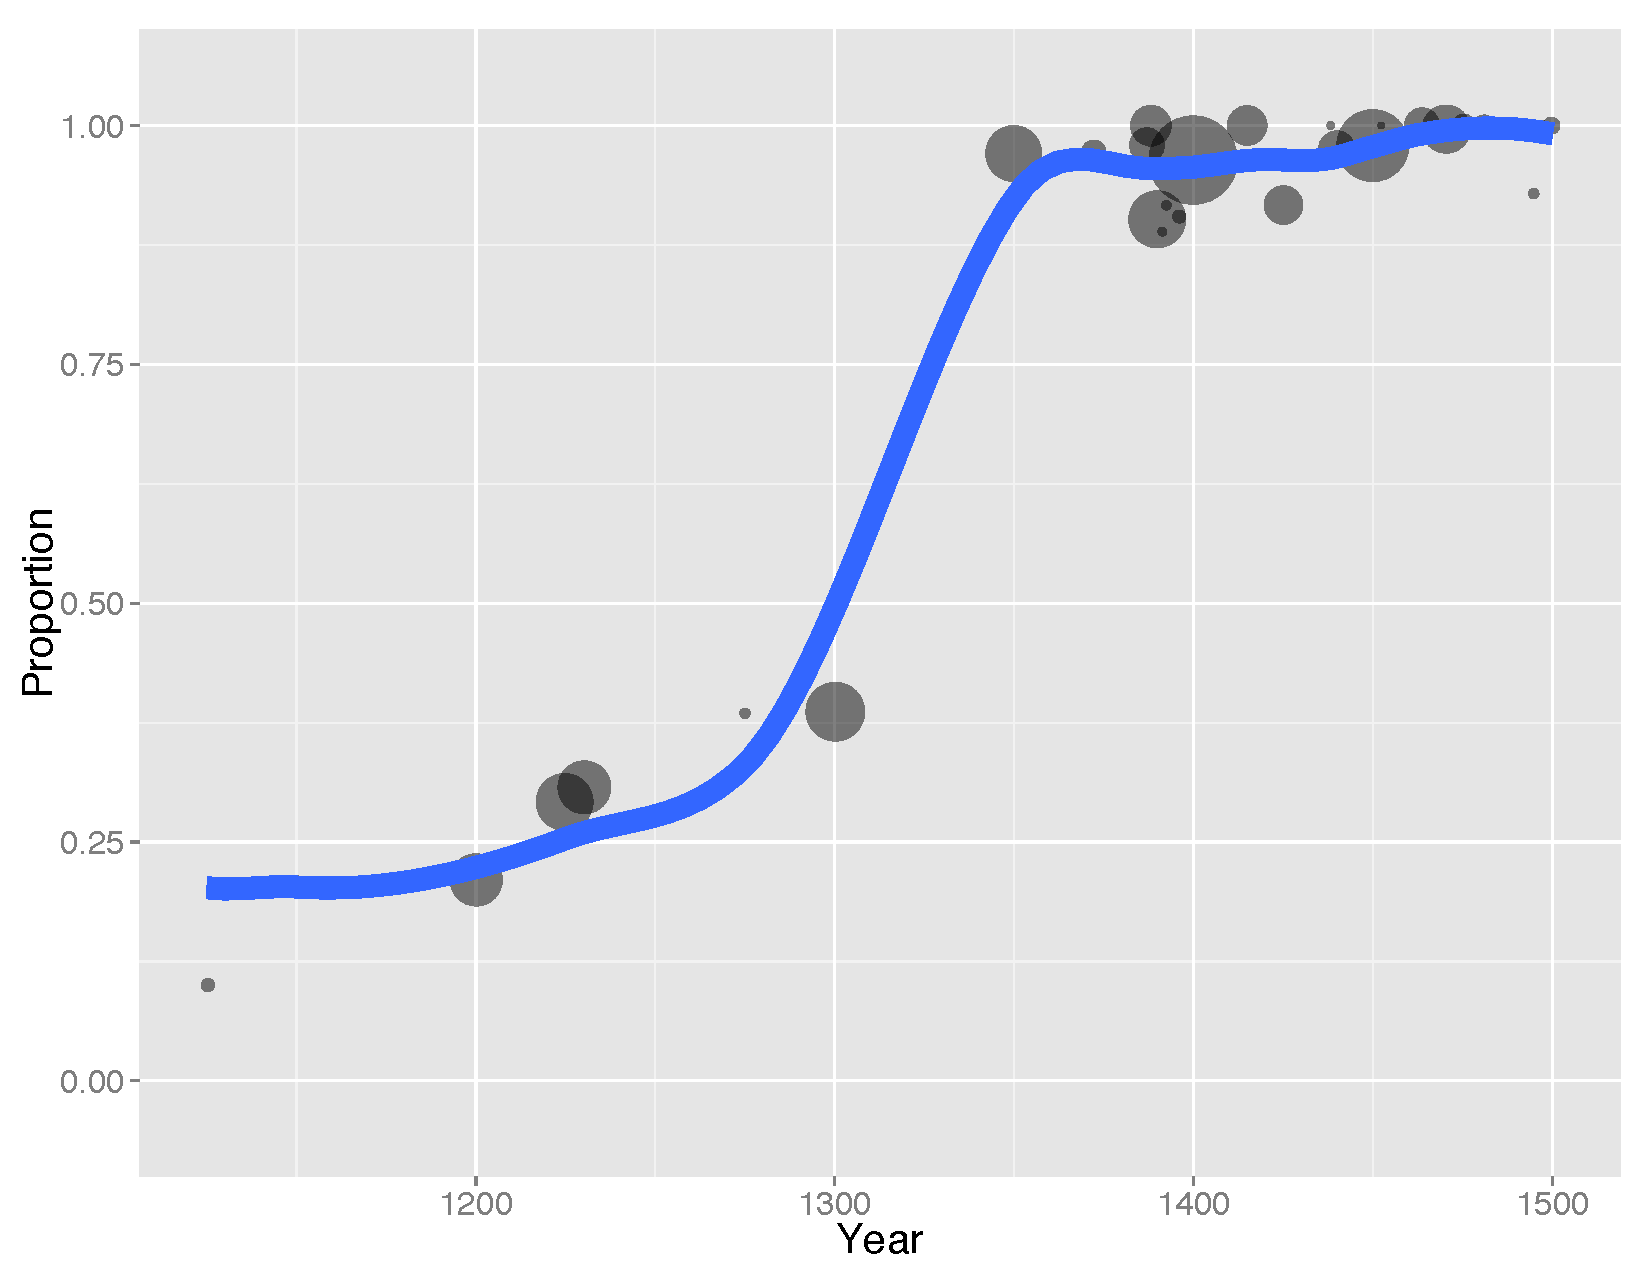
\includegraphics[width=.5\textwidth]{lump-plot1.pdf}\\}
		\only<2>{\emph{\textcolor{red}{ne}} $\rightarrow$ \emph{\textcolor{blue}{(ne...)} \textcolor{mygreen}{not}} }
	\end{center}
%	\vfill \hfill Data from PPCME \citep{ppcme2} 
\end{frame}

%\begin{frame}
%\frametitle{The functional cycle}
%	\begin{center}
%		\only<1>{\textsc{\color{red} neg V} $\rightarrow$ \textsc{\color{blue} neg V neg}}
%		\only<2>{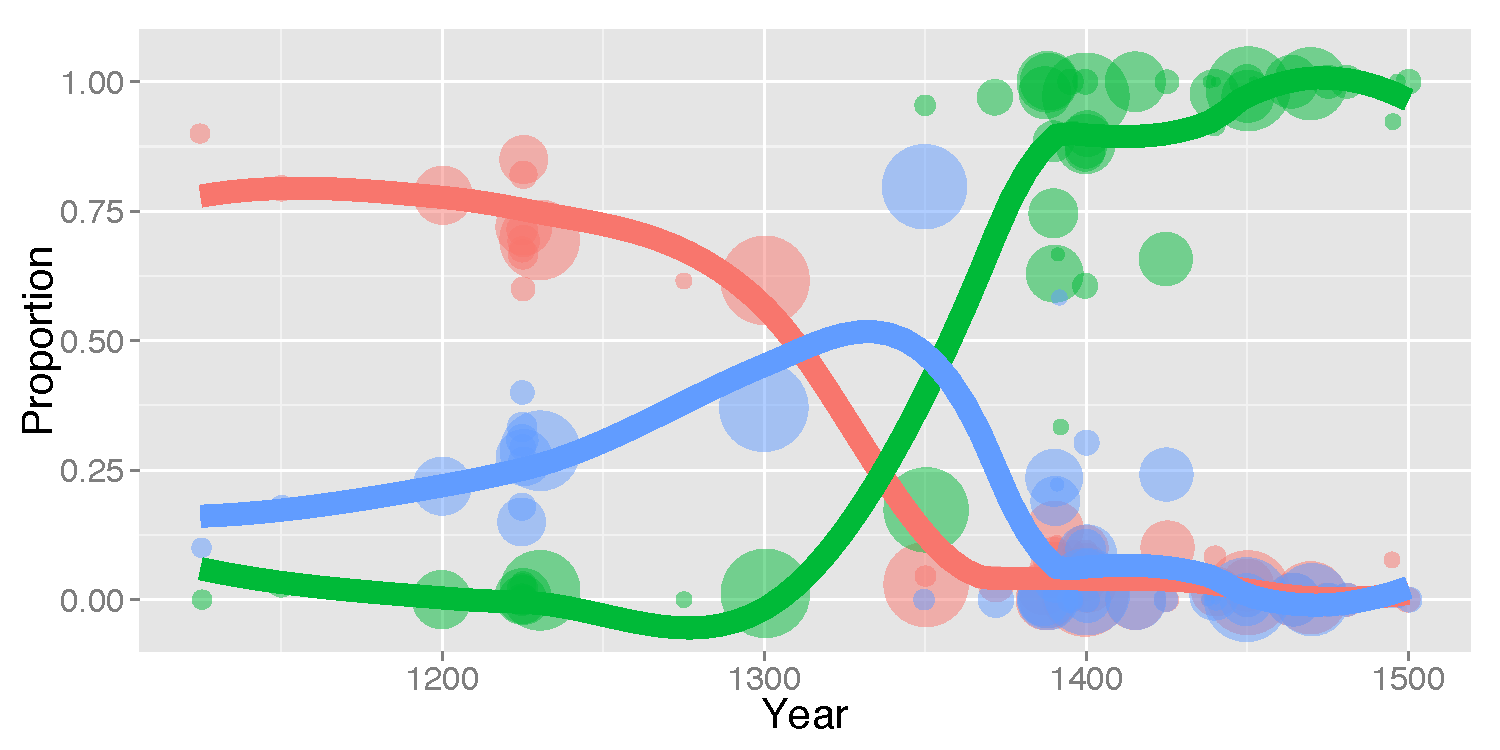
\includegraphics[width=.75\textwidth]{neg-docs-lines.pdf}}
%		\only<3>{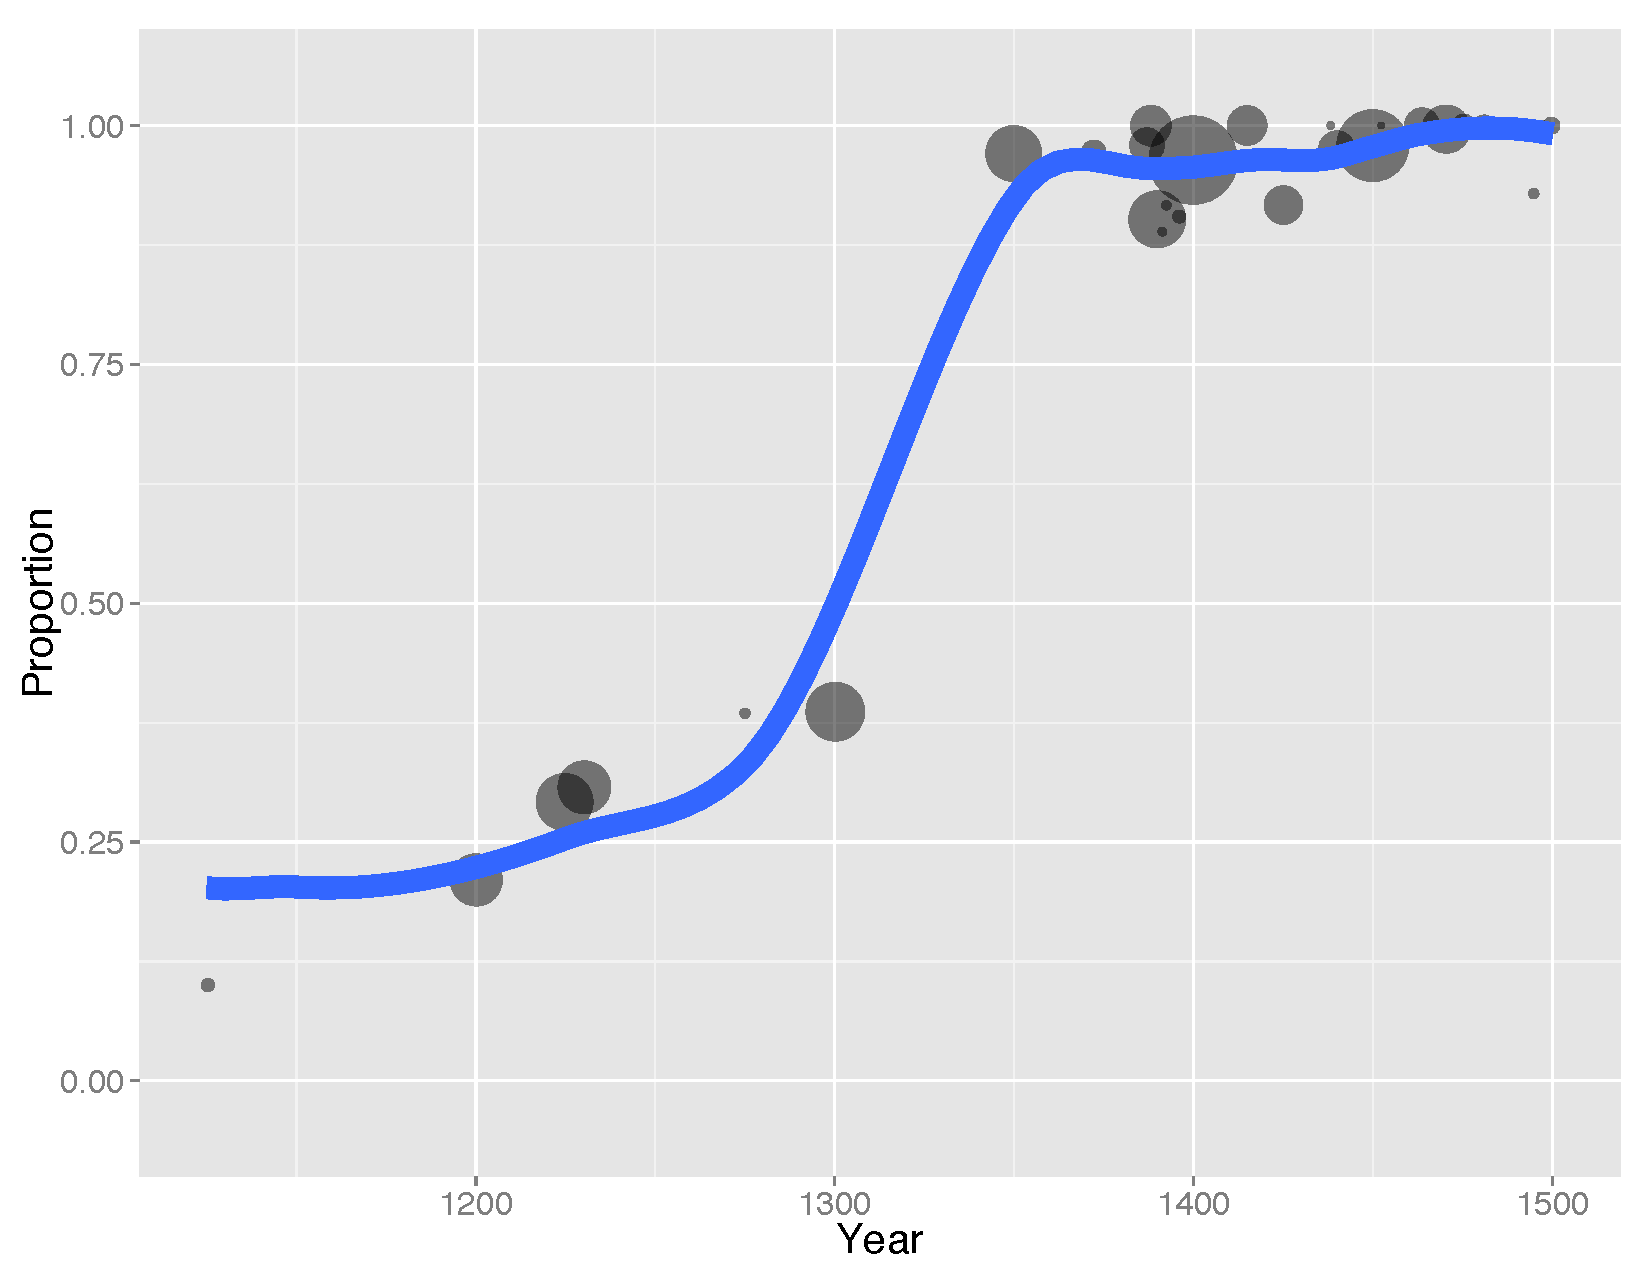
\includegraphics[width=.75\textwidth]{lump-plot1.pdf}}
%	\end{center}
%\end{frame}



%%\begin{frame}{\textsc{\color{red} neg V} $\rightarrow$ \textsc{ \color{blue} neg V neg}}
%%\begin{enumerate}
%%	\item Pragmatic conditions 
%%	\item Experimental evidence
%%	\item Information transmission
%%\end{enumerate}
%%\end{frame}


%\begin{frame}{Emphasis as activation}
%
%\exg. Alle \textipa{D}o men \textipa{D}e swinke\textipa{D} on \textipa{D}essere swinkfulle world, alle he swinke\textipa{D} for sumere hope \textipa{D}e hie habbe\textipa{D}, \textipa{D}e hem oft eaten ande beswink\textipa{D} ... Ac \textipa{D}o \textipa{D}e swinke\textipa{D} for \textipa{D}essere eadi hope, hie \emph{\textcolor{blue}{ne}} bie\textipa{D} \emph{\textcolor{blue}{naht}} becaht \\
%All the men that labour in this toilsome world, all they labour for some hope that they have, that them often at end deceives ... But those that labour for this blessed hope, they \textsc{neg} are not deceived.\\
%"All the men who labor in this toilsome world, they all labor for some hope they have which often \textbf{deceives them} in the end...But those who labor for this blessed hope, \textbf{they are not deceived}."\\ 
%
%    \vfill\hfill (CMVICES,33.385, 1200 CE)
%\end{frame}


\begin{frame}{Emphasis as activation}

\exg. If u ne cnawest e seolf ... If u \emph{\textcolor{blue}{ne}} cnawest \emph{\textcolor{blue}{naut}} e seolf\\
If you not know the self ... If you \textsc{neg} know not the self\\
"If \textbf{you do not know yourself}...If \textbf{you do not know yourself}"\\ 

    \vfill\hfill (CMANCRIW, II.80.941-948, 1230 CE)
\end{frame}


\begin{frame}{Emphasis as activation}

\exg. and te lage hadde to alle te mihtes te haue\textipa{D} nu fulluht for \textipa{D}at clensede te man of sinne: swa do\textipa{D} nu fulluht ac it \emph{\textcolor{blue}{ne}} openede hem \emph{\textcolor{blue}{noht}} te blisse of heuene alse fulcneng do\textipa{D} us.\\
and the law had then all the virtues that has now baptism for that cleansed the man of sin: as does now baptism but it neg opened them not the bliss of heaven as baptism does us.\\
"And \textbf{that rite had then all the virtues which baptism now has}, for that cleansed man of sin even as baptism now does, but \textbf{it opened not to them the bliss of heaven} as baptism does to us."\\

    \vfill\hfill (CMTRINIT, 87.1165, 1225 CE)
\end{frame}


%\begin{frame}{Emphasis as activation}
%
%\exg. Ich nam noht giet sad of mine sines and forti \emph{\textcolor{blue}{ne}} mai ich hie \emph{\textcolor{blue}{noht}} forlete.\\
%I not-am not yet sated of my sins and therefore neg can I them not renounce\\
%``\textbf{I am not yet sated of my sins} and therefore \textbf{I cannot renounce them}."\\
%
%    \vfill\hfill (CMTRINIT, 75.1028, 1225 CE)
%\end{frame}



%\begin{frame}{Emphasis as activation}
%	\begin{itemize}
%		\item \emph{directly activated} : contents have just been explicitly introduced
%		\item \emph{indirectly activated} : contents can be inferred
%		\item \emph{non-activated} : otherwise
%	\end{itemize}
%%A proposition is \emph{directly activated} if its contents have just been explicitly introduced into the discourse, so it is present to the joint attention of speakers and hearers. A proposition is \emph{indirectly activated} if its contents can be inferred from the discourse either via an entailment or implicature.  A proposition is \emph{non-activated} if its contents have not been explicitly introduced into the discourse or it cannot be inferred from the preceding discourse.
%    \vfill \hfill \footnotesize{\citep{schwenter2006,hansen-visconti2009,hansen-visconti2012,wallage2013}}
%\end{frame}



\begin{frame}
\frametitle{Emphasis as activation}

\begin{center}
\begin{tikzpicture}
%\node[visible on=<1->] (left) at (-1, 2)    {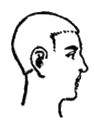
\includegraphics[width=.15\textwidth]{left.jpg}};
%\node[visible on=<1->] (left) at (7, 2)    {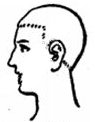
\includegraphics[width=.15\textwidth]{right.jpg}};
%draw horizontal line
\draw[visible on=<1->] (0,0) -- (8,0);
%draw ticks
\draw[visible on=<1->] (0,3pt) -- (0,-3pt);
\draw[visible on=<1->] (4,3pt) -- (4,-3pt);
\draw[visible on=<1->] (8,3pt) -- (8,-3pt);
%draw tick labels
\draw[text width=2cm,align=center,visible on=<2->] (8,0) node[below=3pt] {\textsc{directly activated} } ;
\draw[text width=2cm,align=center,visible on=<3->] (4,0) node[below=3pt] {\textsc{indirectly activated} } ;
\draw[text width=2cm,align=center,visible on=<4->] (0,0) node[below=3pt] {\textsc{non-activated} } ;
%
\draw [ultra thick,blue, visible on=<5>] (7,.5) to (8,.5);
\draw (7.5,1) node[visible on=<5>] {\textsc{\color{blue} neg V neg}};
%
\draw [ultra thick,blue, visible on=<6>] (5,.5) to (8,.5);
\draw (6.5,1) node[visible on=<6>] {\textsc{\color{blue} neg V neg}};
%
\draw [ultra thick,blue, visible on=<7>] (3,.5) to (8,.5);
\draw (5.5,1) node[visible on=<7>] {\textsc{\color{blue} neg V neg}};
%
\draw [ultra thick,blue, visible on=<8>] (0,.5) to (8,.5);
\draw (4,1) node[visible on=<8>] {\textsc{\color{blue} neg V neg}};

\end{tikzpicture}     
\end{center}

\only<1-4>{\vfill \hfill (\cite{dryer1996}, cf. \cite{chafe1974,prince1981})}
\only<5->{\vfill \hfill \footnotesize{\citep{hansen-visconti2009,hansen-visconti2012,wallage2013}}}
\end{frame}


\begin{frame}
\frametitle{Experimental evidence on activation}

  \begin{center}
    \begin{tikzpicture}
      \node[visible on=<1->] at (0,0)      {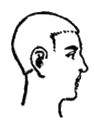
\includegraphics[width=.15\textwidth]{left.jpg}};
      \node[visible on=<1-2>] at (8,0) {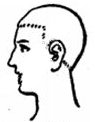
\includegraphics[width=.15\textwidth]{right.jpg}};
      \node[align=center,visible on=<2>] at (4,0) {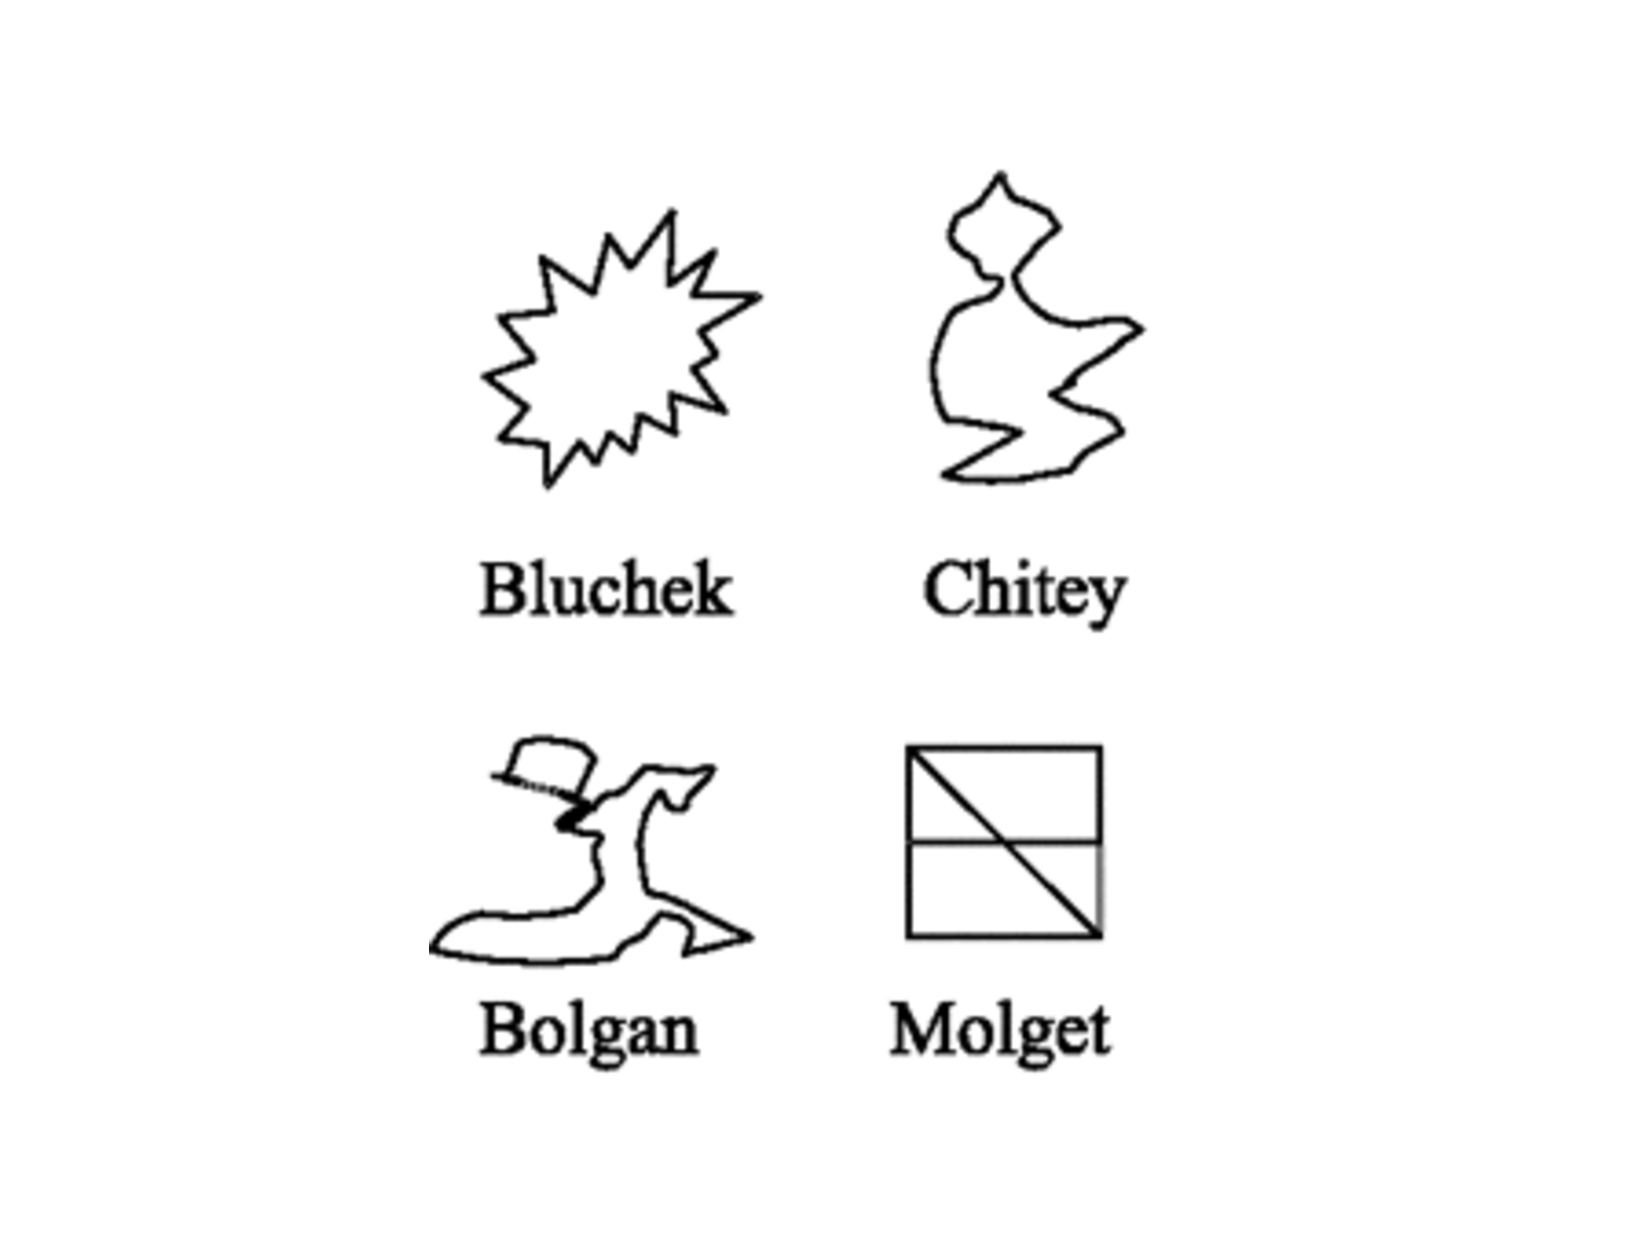
\includegraphics[width=5cm]{wu-keysar-shared.pdf}};
      \node[align=center,visible on=<3>] at (4,0) {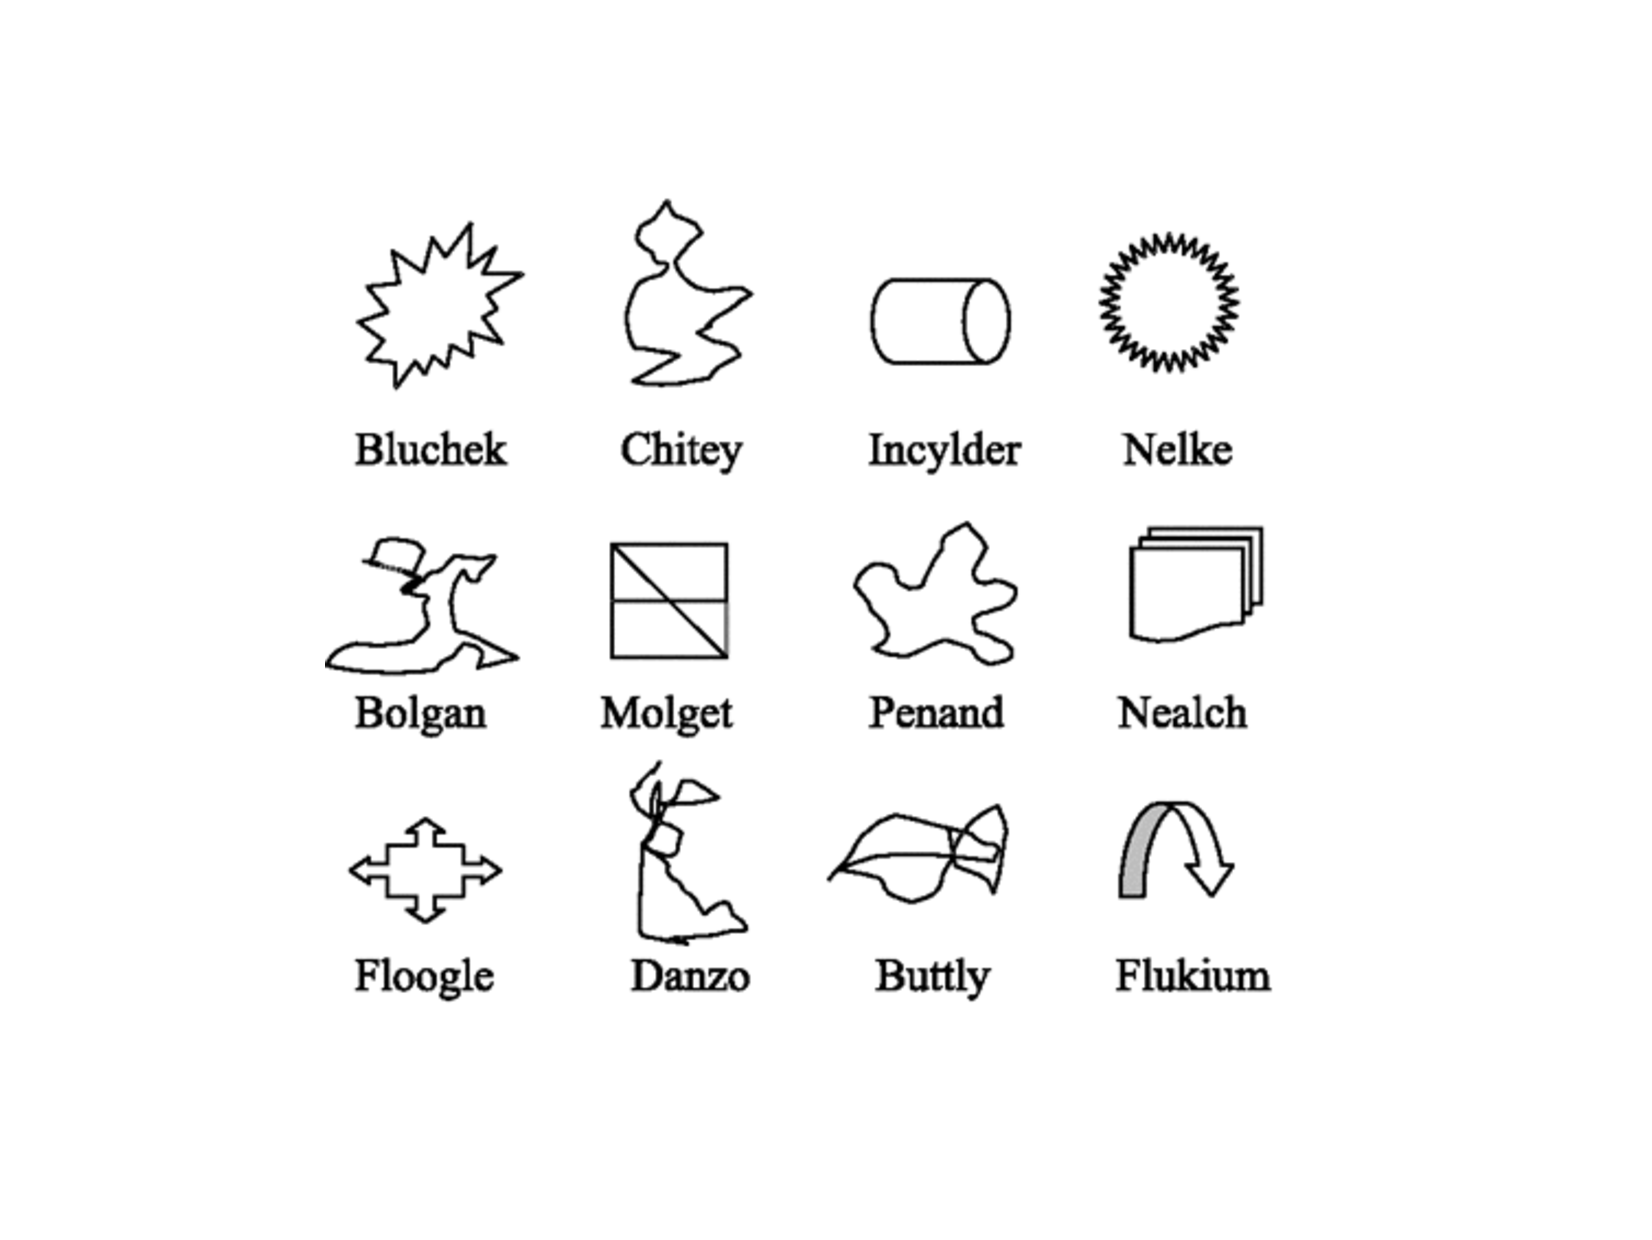
\includegraphics[width=5cm]{wu-keysar-names.pdf}};      
      \node[visible on=<4-9>] at (8,0) {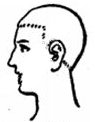
\includegraphics[width=.15\textwidth]{right.jpg}};
      \node[visible on=<4-6>] at (0,-3) {
\includegraphics[width=3cm]{blucheck.pdf}};
      \path[->] (1,-1)  edge[dashed, out=-35,in=220, visible on=<5-6>] node[below, text width=3cm, align=center]  { bluchek } (7,-1);
	\node[visible on=<6>] at (8,-3) {
\includegraphics[width=3cm]{blucheck.pdf}};      
	\node[visible on=<7-9>] at (0,-3) {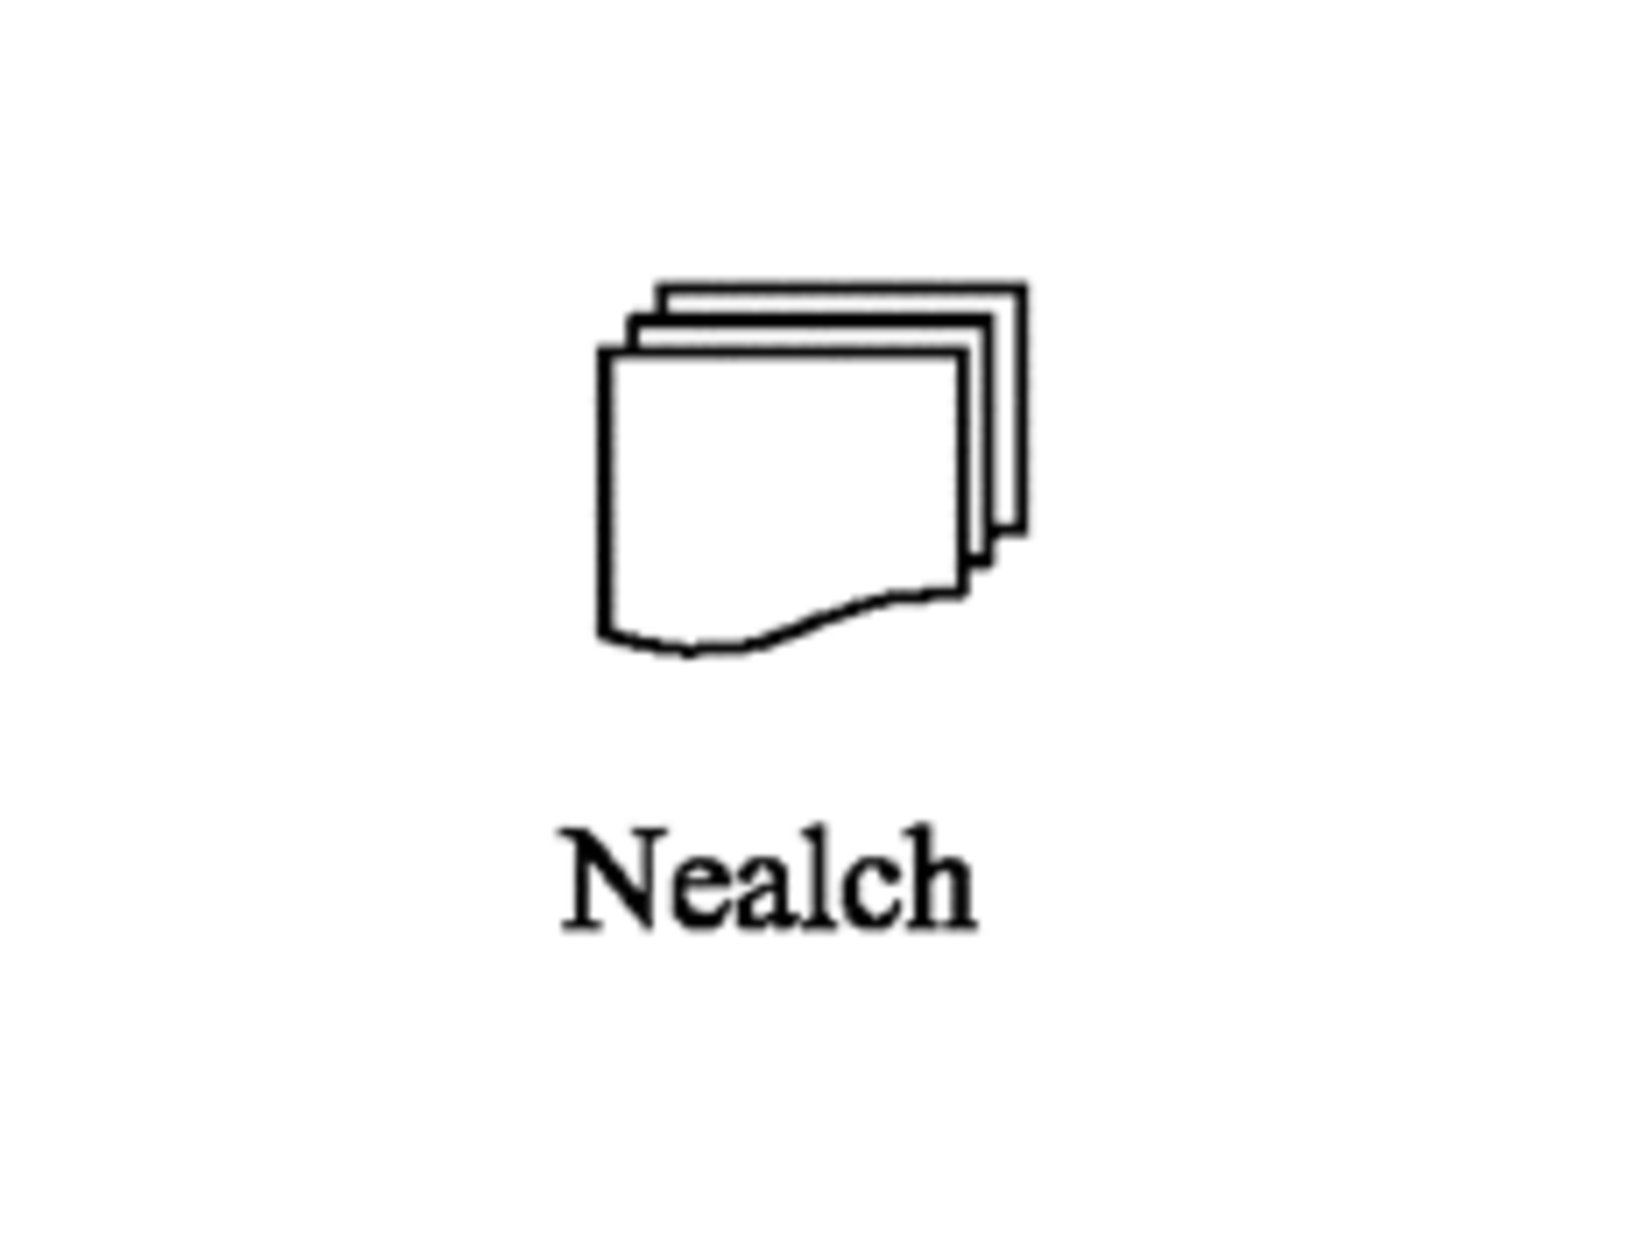
\includegraphics[width=3cm]{nealch.pdf}};
      \path[->] (1,-1)  edge[dashed, out=-35,in=220, visible on=<8-9>] node[below, text width=3cm, align=center]  { nealch } (7,-1);
	\node[visible on=<9>] at (8,-3) {?};     
	 \node[align=center,visible on=<10>] at (5,0) {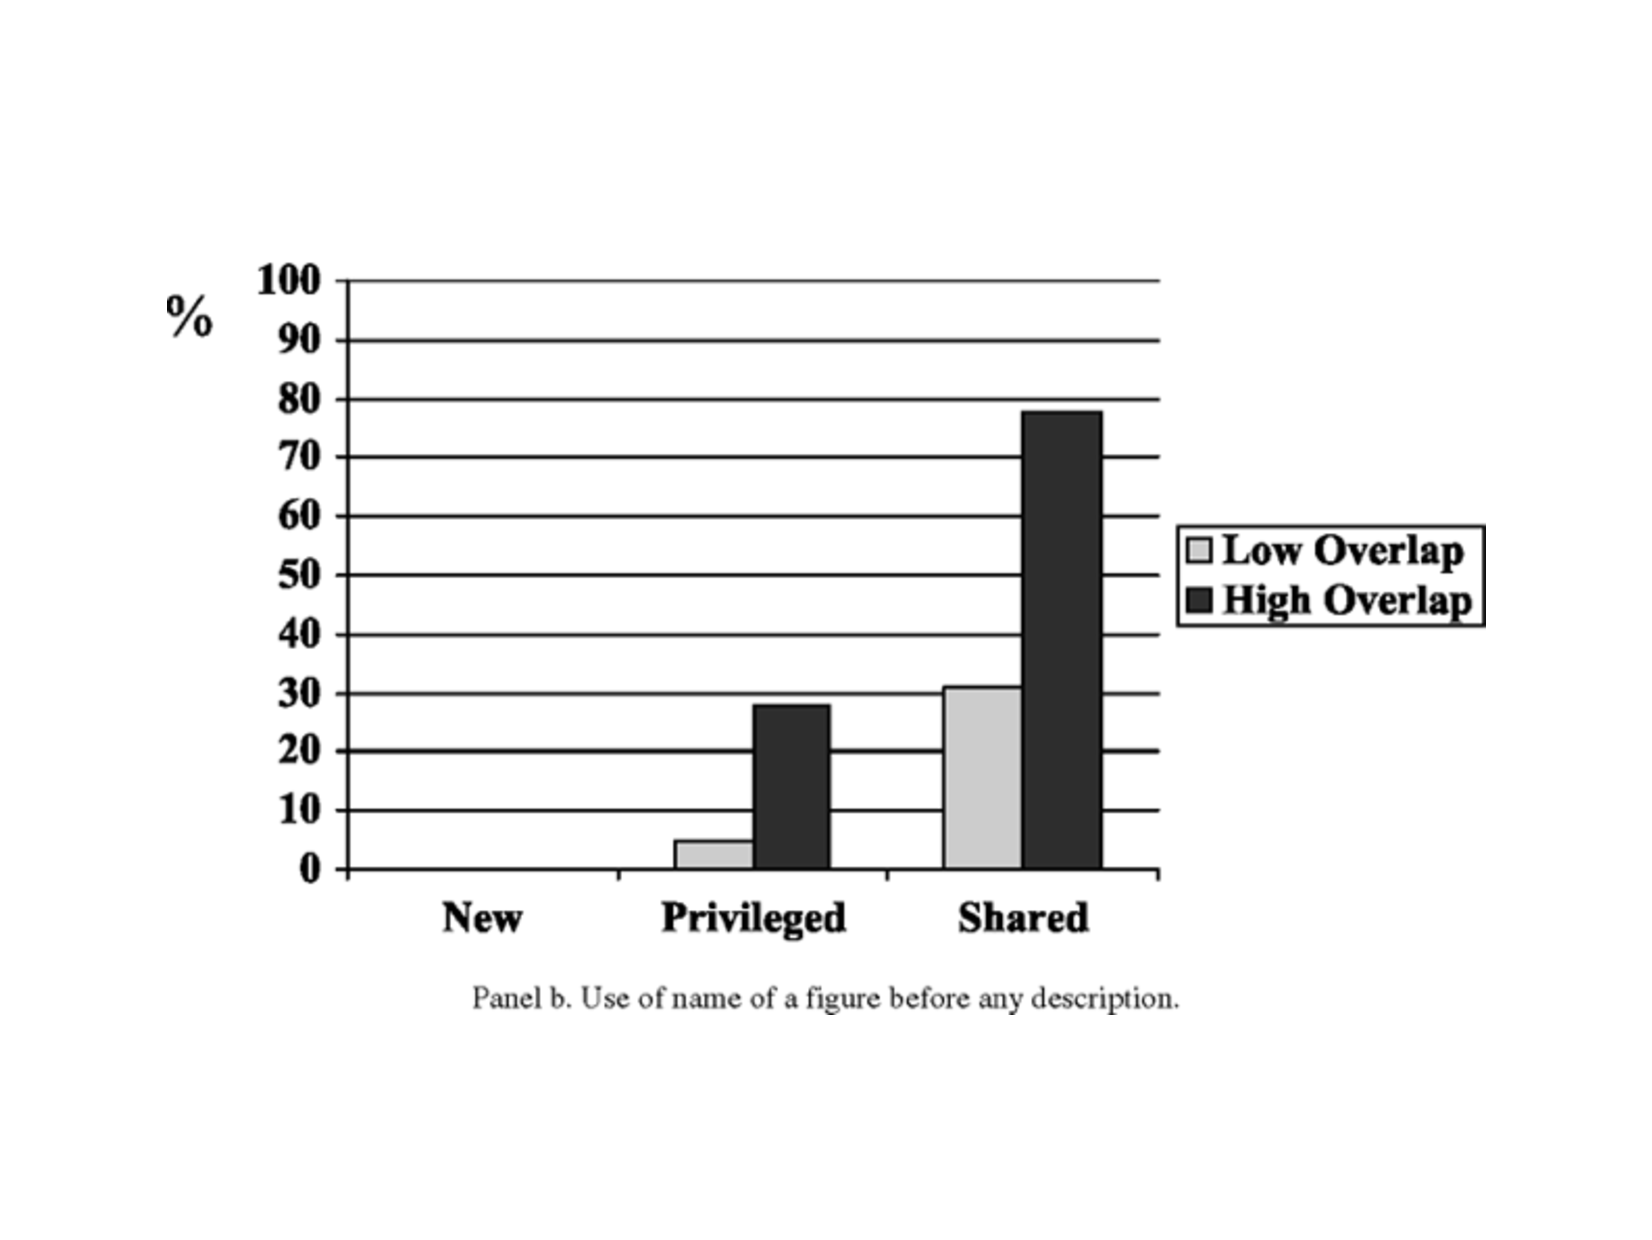
\includegraphics[width=6.5cm]{wu-keysar.pdf}};
    \end{tikzpicture}
  \end{center}
	     \vfill \hfill \citep{wu-keysar2007}
\end{frame}


%\begin{frame}
%\frametitle{Experimental evidence on activation}
%\only<2>{Speakers' privileged information leaks into what they say:}
%     \begin{center}
%	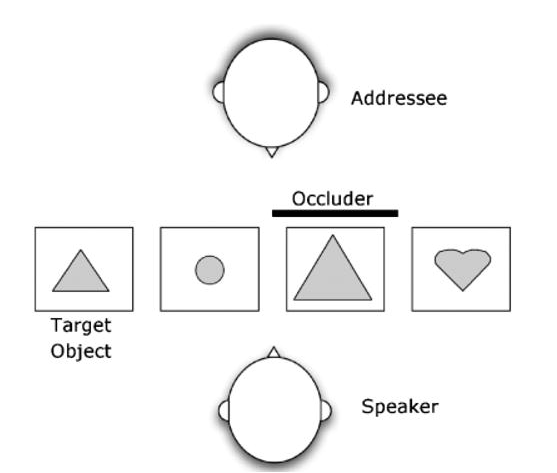
\includegraphics[width=2in]{elephants-exp.png}  	\only<2>{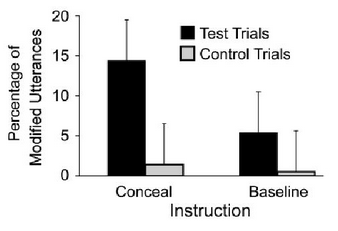
\includegraphics[width=2in]{elephant-results.png}}
%     \end{center}
%	     \vfill \hfill \citep{lane-etal2006}
%\end{frame}


\begin{frame}{The activation signaling game}
  \begin{center}
    \begin{tikzpicture}
      \node[visible on=<1->] (left)      {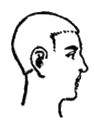
\includegraphics[width=.15\textwidth]{left.jpg}};
      \node[visible on=<1->] (right) [right=4cm  of left] {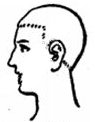
\includegraphics[width=.15\textwidth]{right.jpg}};
      \node[visible on=<2->] (G1) [draw,above=.25cm of left] {$t \in T$};
%      \node[visible on=<4-9>] (t) [above=.25cm of G1] {$t_0 : $ \textsc{discourse new}};
      \node[visible on=<3->] (S) [draw,below=.25cm of left] {$s : \mathcal{P}(T) \rightarrow M$};
      \path[->] (left)  edge[dashed, out=-35,in=220, visible on=<4->] node[below, text width=3cm, align=center]  { \{ \textcolor{red}{$m_1$}, \textcolor{blue}{$m_2$} \} } (right);
      \node[visible on=<5->] (R) [draw,below=.25cm of right] {$r : M \rightarrow A$};
      \node[visible on=<6->] (G2) [draw,above=.25cm of right] {$a \in A$};
%      \node[visible on=<9>] (a) [above=.25cm of G2] {$a_0 : $ \textsc{discourse new}};
%      \node[visible on=<10->] (t) [above=.25cm of G1] {$t_1 : $ \textsc{discourse old}};
    \end{tikzpicture}
  \end{center}
\end{frame}


\begin{frame}{The activation signaling game}
Bias parameter, $b$, encodes tendency to overestimate activation:
  \begin{center}
	\begin{equation}
	 U_S(t,a) = 1 - (a - t - (1-t)b)^2
	\end{equation}

	\begin{equation}
	 U_R(t,a) = 1 - (a - t)^2	
	\end{equation}
  \end{center}
  \vfill \hfill \citep{crawford-sobel:1982}
\end{frame}


\begin{frame}{The equilibria of the signaling game}
\emph{Evolutionarily stable strategies} are jointly strict maxima of expected utilities:
  \begin{center}
	\begin{equation}
	 E[U_S(s,r)] = \int_T [1 - (r(s(t)) - t - (1-t)b)^2]p(t)dt
	\end{equation}

	\begin{equation}
	 E[U_R(s,r)] = \int_T [1 - (r(s(t)) - t)^2	]p(t)dt
	\end{equation}
  \end{center}
  \vfill \hfill  \citep{selten:1980}
\end{frame}


\begin{frame}
\frametitle{The equilibria of the signaling game}
Prior probability distribution estimated from PPCME \citep{ppcme2} by \citet{wallage2013}:
\vfill
\resizebox{\textwidth}{!}{% 
\begin{tabular}{@{}cccc@{}}
\hline
    \textsc{period}   &\textsc{non-activated} & \textsc{indirectly activated} & \textsc{directly activated} \\
\hline
1150-1250    & 393  & 203 & 52   \\
1250-1350    & 346  & 296 & 42 \\
1350-1420    & 294  & 179 & 60 \\ \hline
\textsc{total} &1033 & 678 & 154  \\
\end{tabular}
}
\vfill \hfill (cf. \cite{tottie:1991,thompson1998})
\end{frame}


\begin{frame}
\frametitle{The equilibria of the signaling game}
Prior probability distribution as a beta distribution $\mathcal{B}(1,2)$:
	\begin{center}
		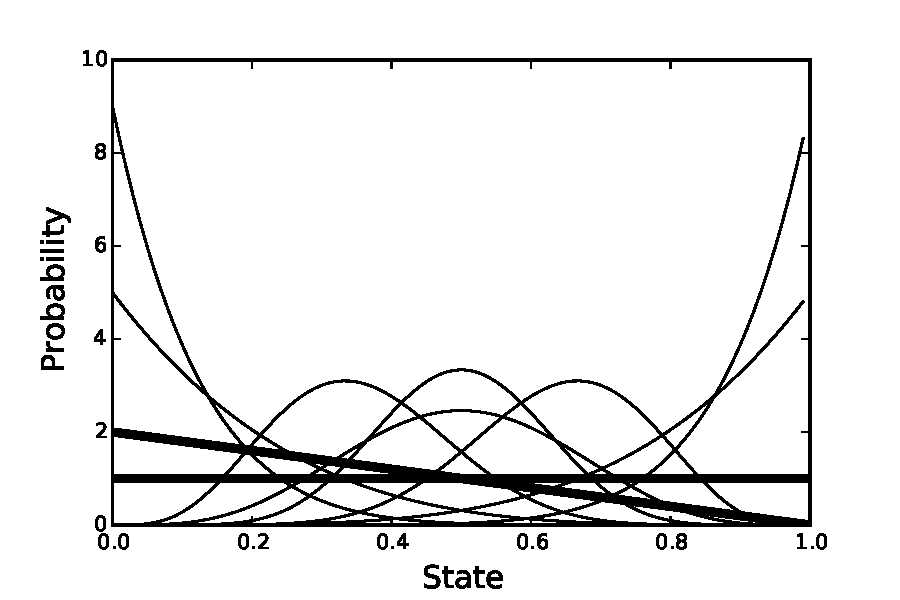
\includegraphics[width=.75\textwidth]{beta-distribution.pdf}
	\end{center}
\end{frame}

\begin{frame}
\frametitle{The equilibria of the signaling game}
Evolutionarily stable speaker and hearer strategies as a function of the amount of speaker bias:
	\begin{center}
		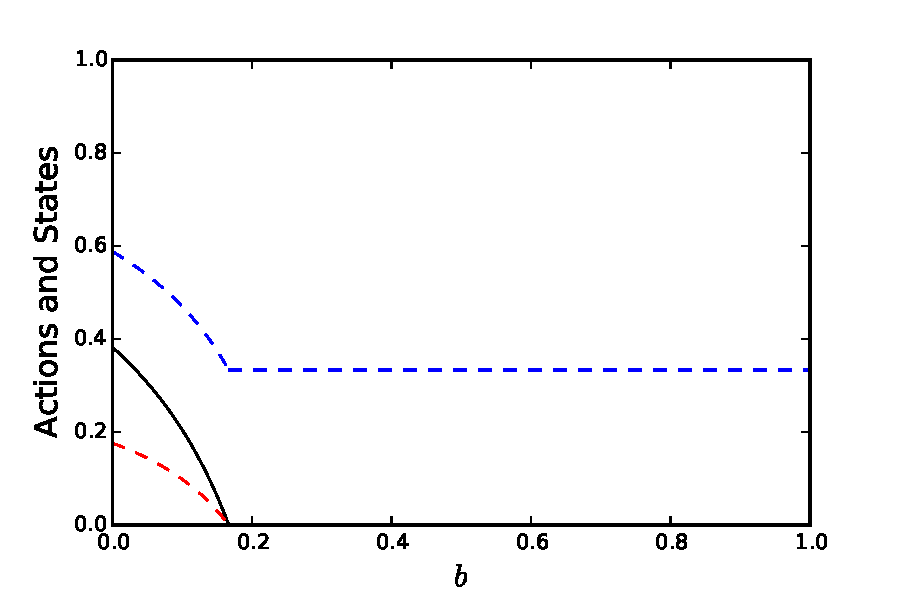
\includegraphics[width=.7\textwidth]{sol2-beta.pdf}
	\end{center}
	\only<2>{\vfill \hfill  \footnotesize{No equilibria are \emph{neologism proof} \citep{farrell:1993}}}
\end{frame}


\begin{frame}
\frametitle{The dynamics of signaling activation}
Simulations of population from same starting state with different degrees of sender bias:
	\begin{center}
		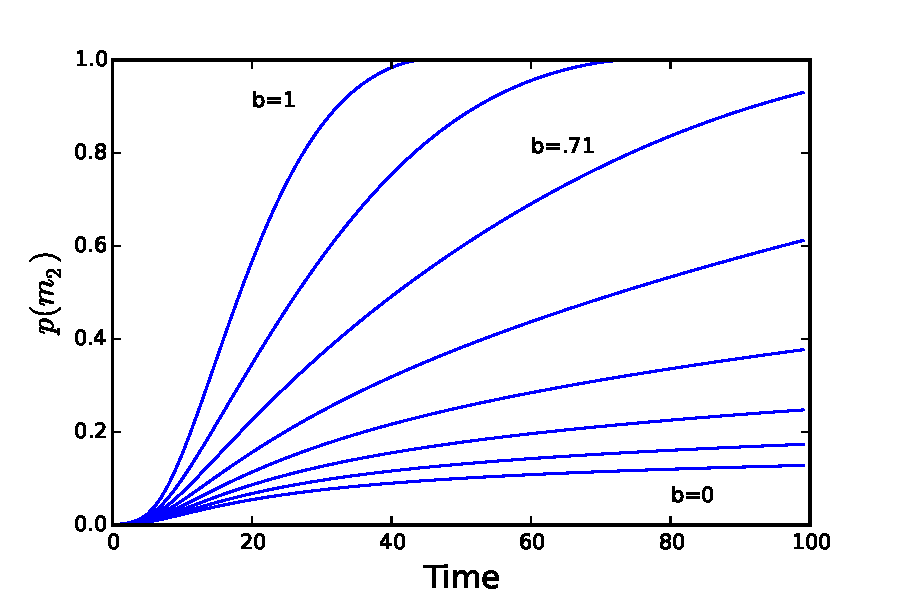
\includegraphics[width=.75\textwidth]{replicator-multiple-b-eps-converted-to.pdf}
	\end{center}
	\vfill \hfill \footnotesize{(\emph{Replicator dynamics}: \cite{taylor-jonker:1978,borgers-sarin1997})}
\end{frame}


\begin{frame}
\frametitle{Modeling the dynamics of signaling activation}
Model fit to corpus data:
	\begin{center}
		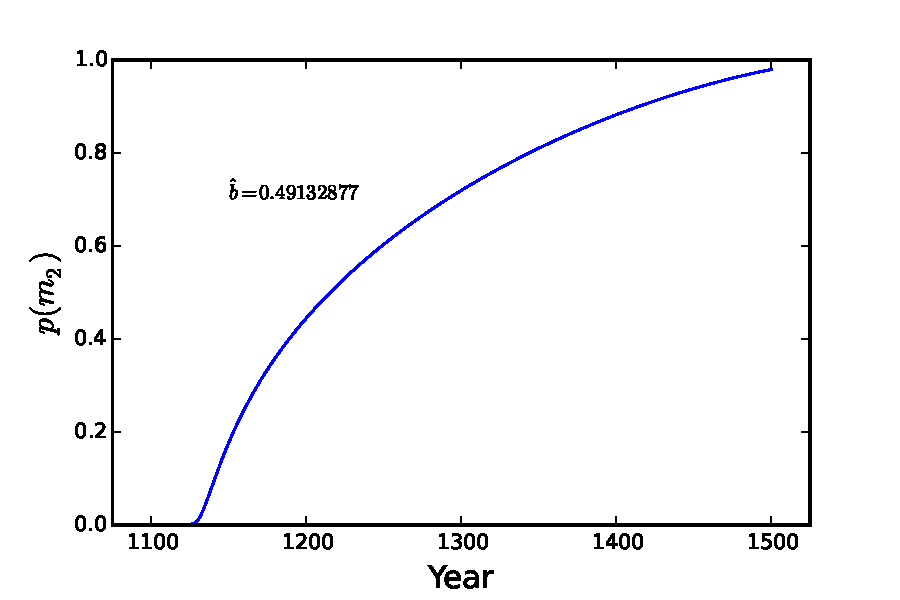
\includegraphics[width=.75\textwidth]{m2-sol.pdf}
	\end{center}
	\only<2>{\vfill \hfill $E[b] \in (.1398, .3549)$ estimated from \citet{wu-keysar2007}}
\end{frame}


\begin{frame}
\frametitle{Modeling the dynamics of signaling activation}
Information-theoretic bleaching of \textcolor{blue}{$m_2$}:
	\begin{center}
		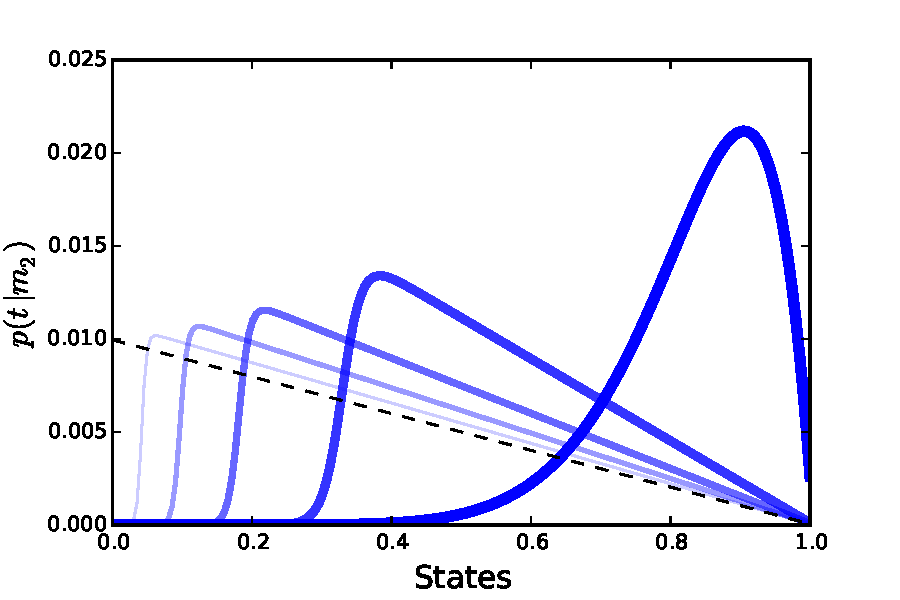
\includegraphics[width=.7\textwidth]{pt-m2.pdf}
	\end{center}
	\only<2>{\emph{To emphasize everything is to emphasize nothing} \footnotesize{\citep{kiparsky-condoravdi:2006}}}
	\only<1>{\vfill \hfill (cf. \cite{kullback-leibler1951divergence})}
%	\vfill \hfill $\hat{b} = 0.49132877$
\end{frame}


\begin{frame}
\frametitle{Modeling the dynamics of signaling activation}
The functional cycle as a push chain:
	\begin{center}
		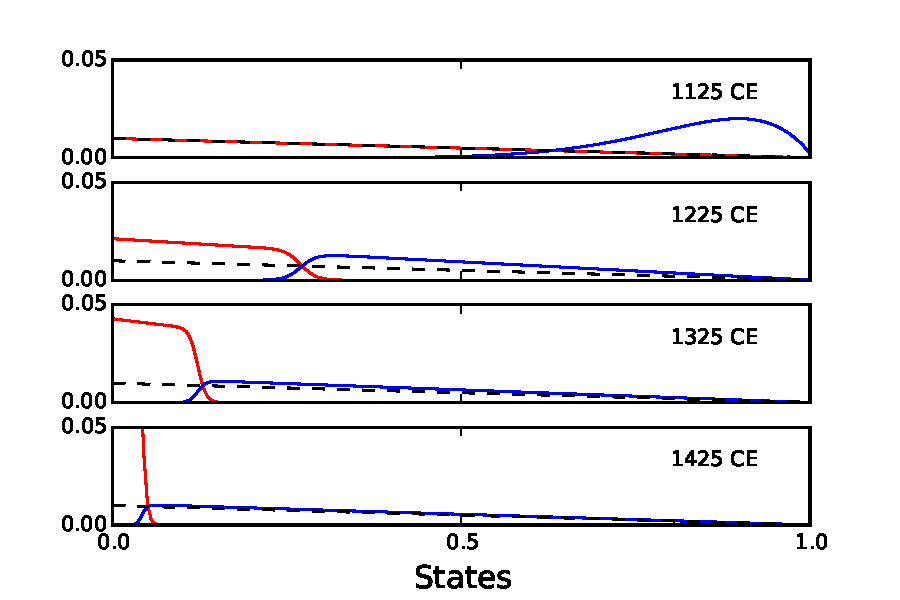
\includegraphics[width=.75\textwidth]{push-chain.pdf}
	\end{center}
	\vfill \hfill (cf. \cite{wallage2013})
\end{frame}

\begin{frame}
\frametitle{The functional cycle}
	\begin{center}
		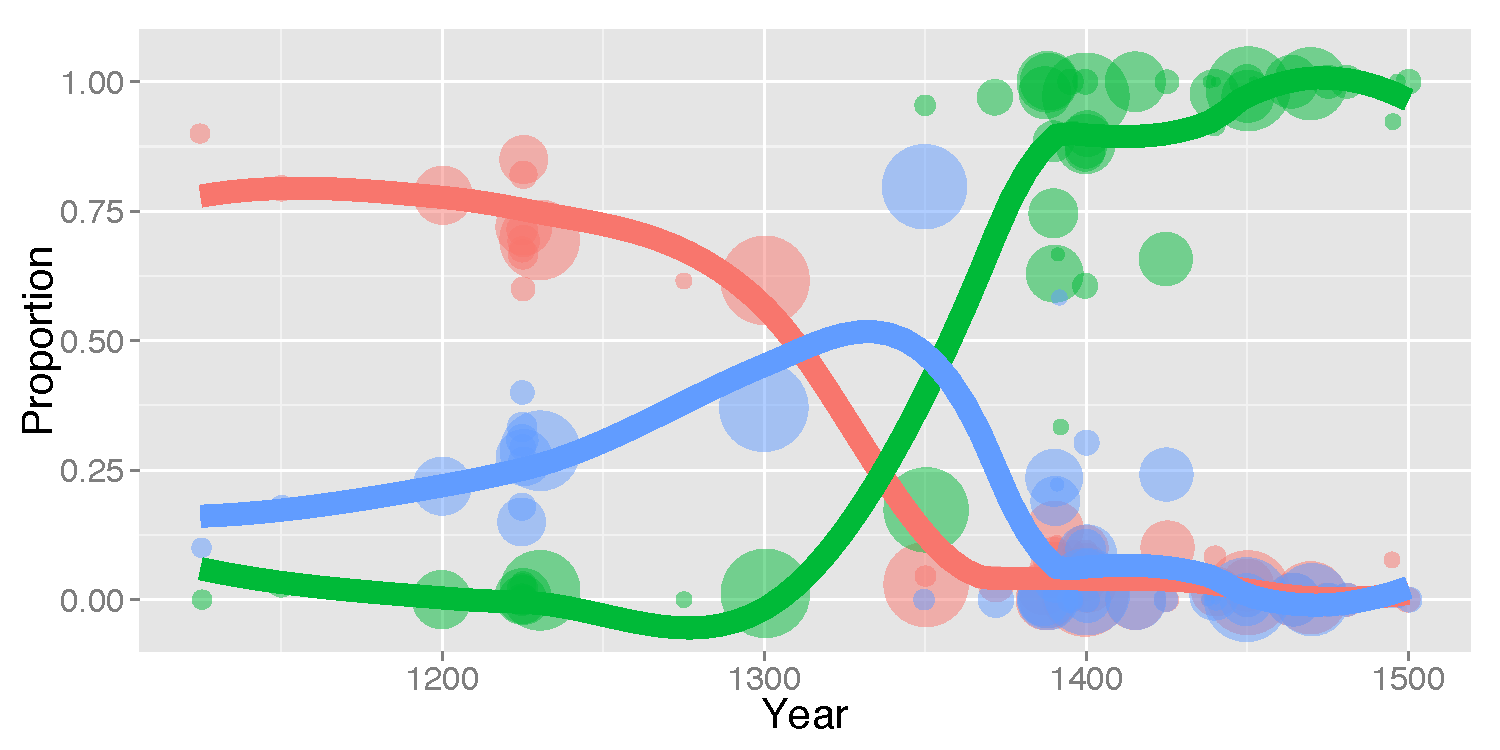
\includegraphics[width=.75\textwidth]{neg-docs-lines.pdf}\\
		\emph{\textcolor{red}{ne}} $\rightarrow$ \emph{\textcolor{blue}{ne...not}} $\rightarrow$ \emph{\textcolor{mygreen}{not}}
	\end{center}
\end{frame}

%%%%%%%%%%%%%%%%%%%%%%%%%%%%%%%%%%%%%%%%%%%%%%%%%
\section{The formal cycle}

\begin{frame}
\frametitle{The formal cycle}
	\begin{center}
		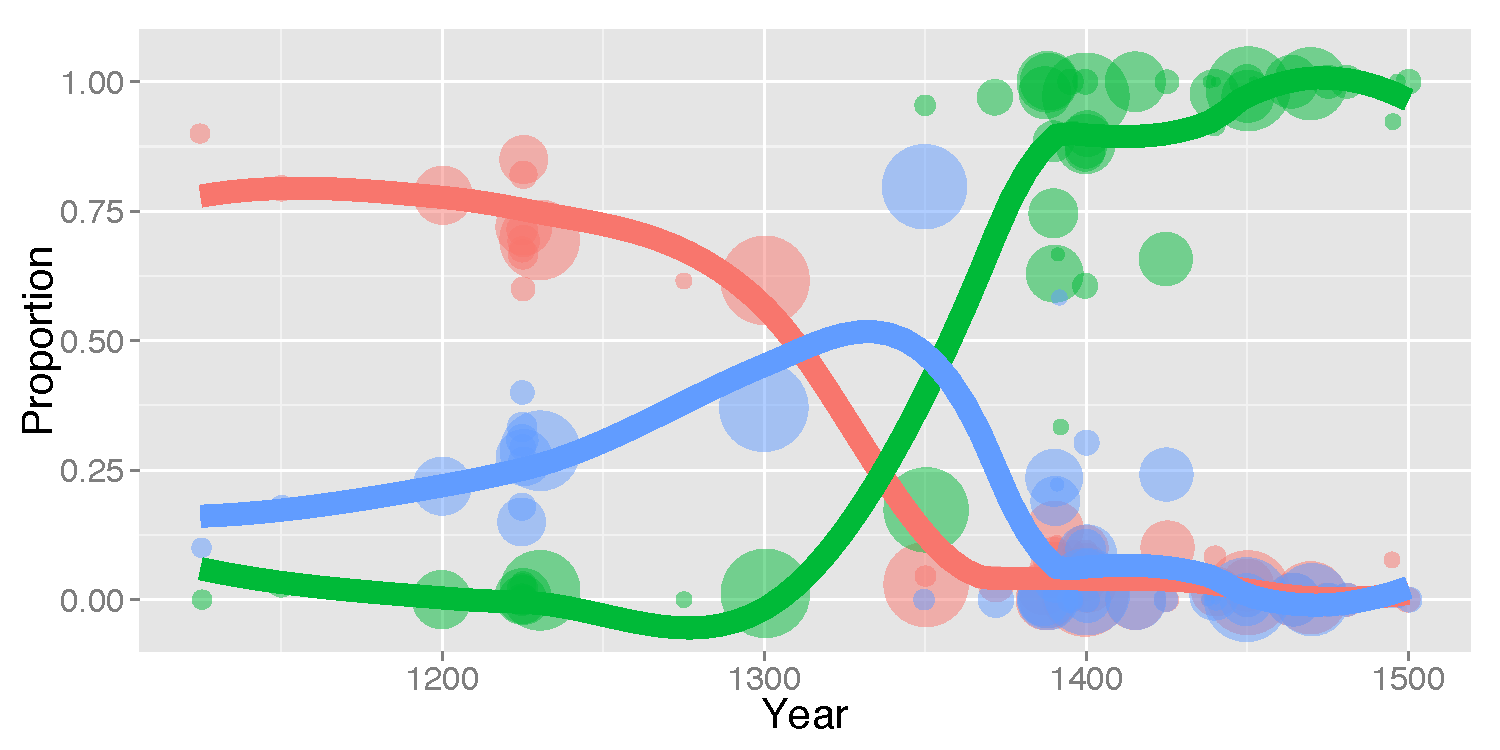
\includegraphics[width=.75\textwidth]{neg-docs-lines.pdf}\\
		\emph{\textcolor{red}{ne}} $\rightarrow$ \emph{\textcolor{blue}{ne...not}} $\rightarrow$ \emph{\textcolor{mygreen}{not}}
	\end{center}
%	\vfill \hfill Data from PPCME \citep{ppcme2} 
\end{frame}

%\begin{frame}
%\frametitle{The formal cycle}
%	\begin{center}
%		\only<1>{\textsc{\color{red} neg V neg} $\rightarrow$ \textsc{\color{blue} neg V neg} $\rightarrow$ \textsc{\color{green} V neg}}
%		\only<2>{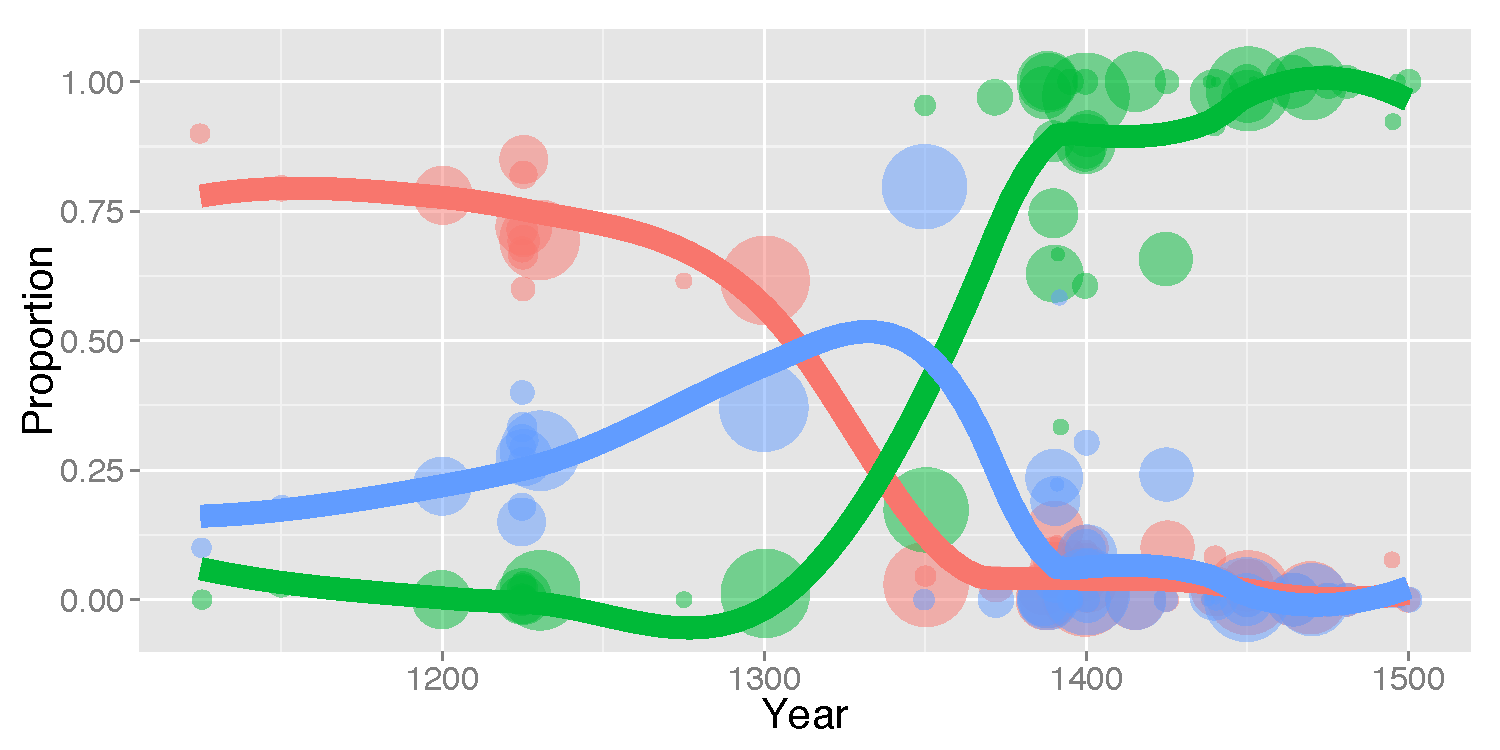
\includegraphics[width=.75\textwidth]{neg-docs-lines.pdf}}
%		\only<3>{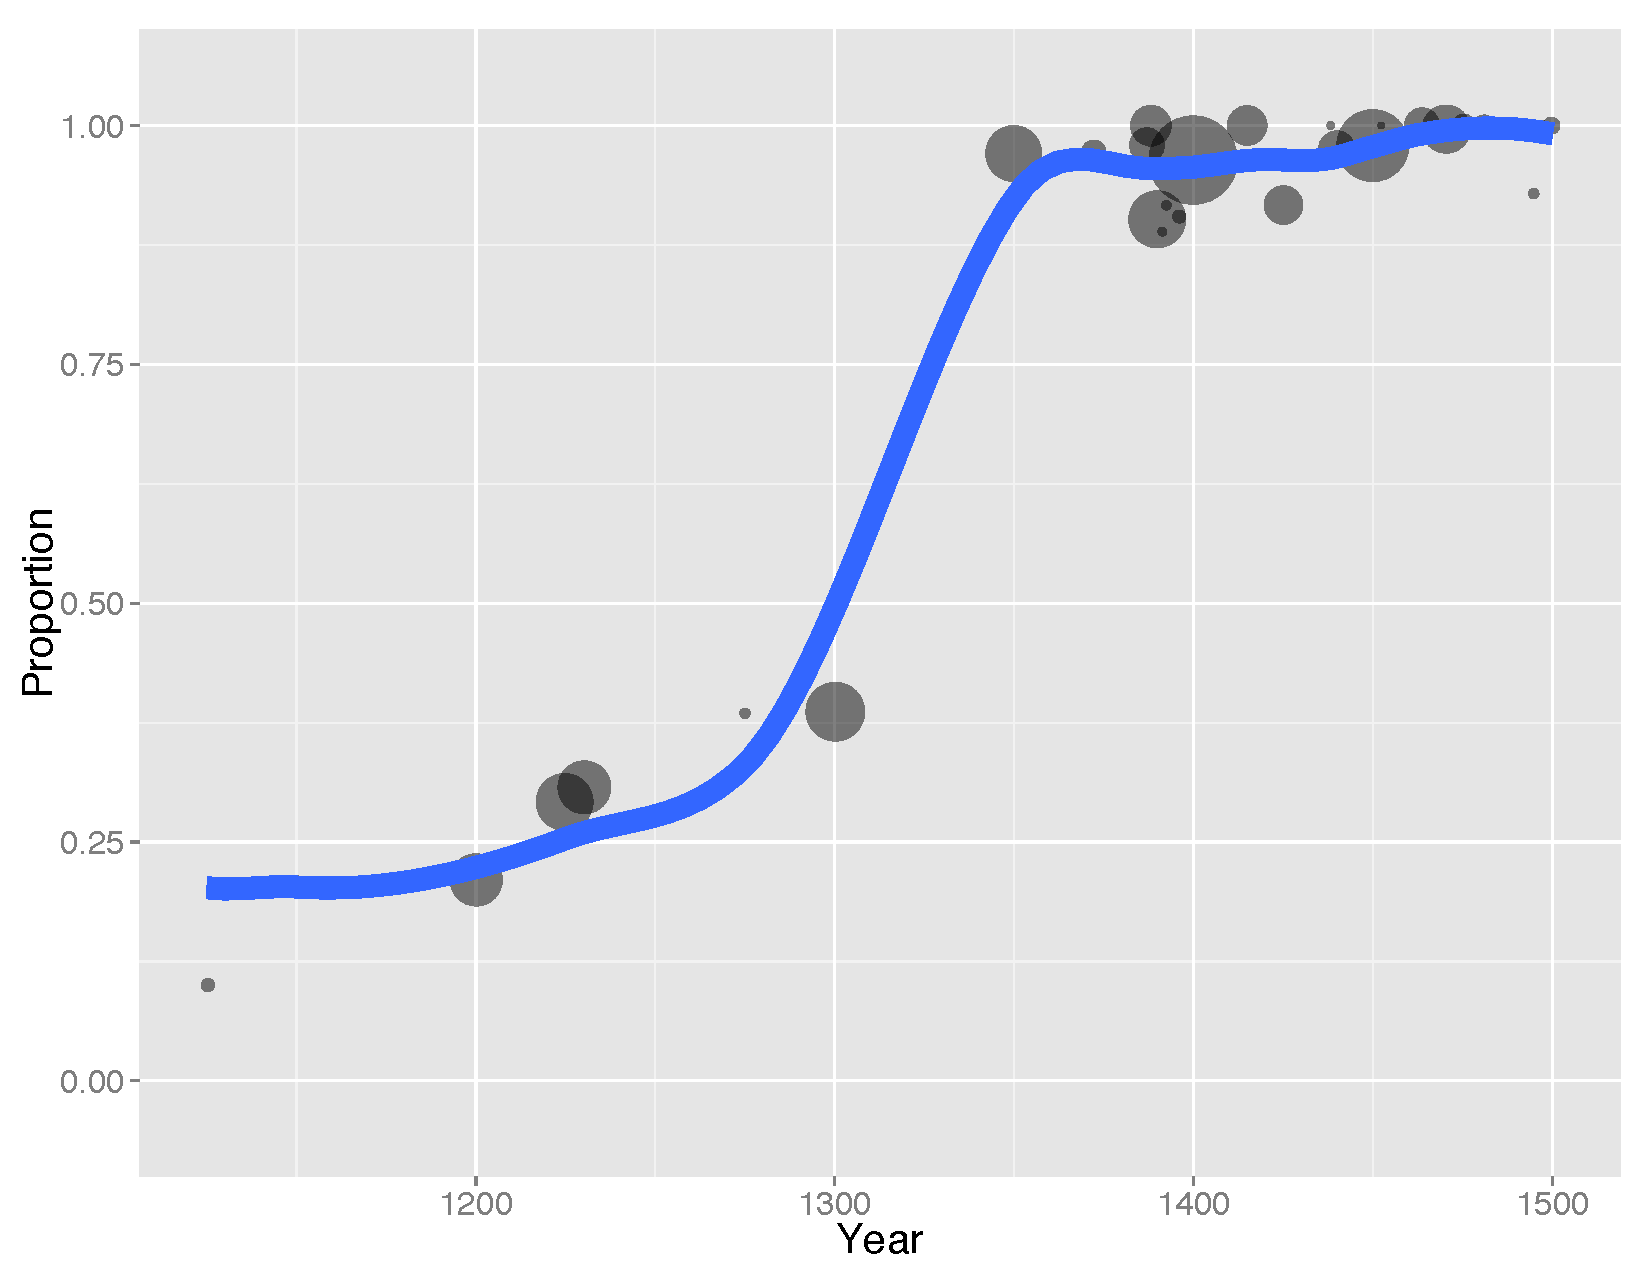
\includegraphics[width=.75\textwidth]{lump-plot1.pdf}}
%		\only<4>{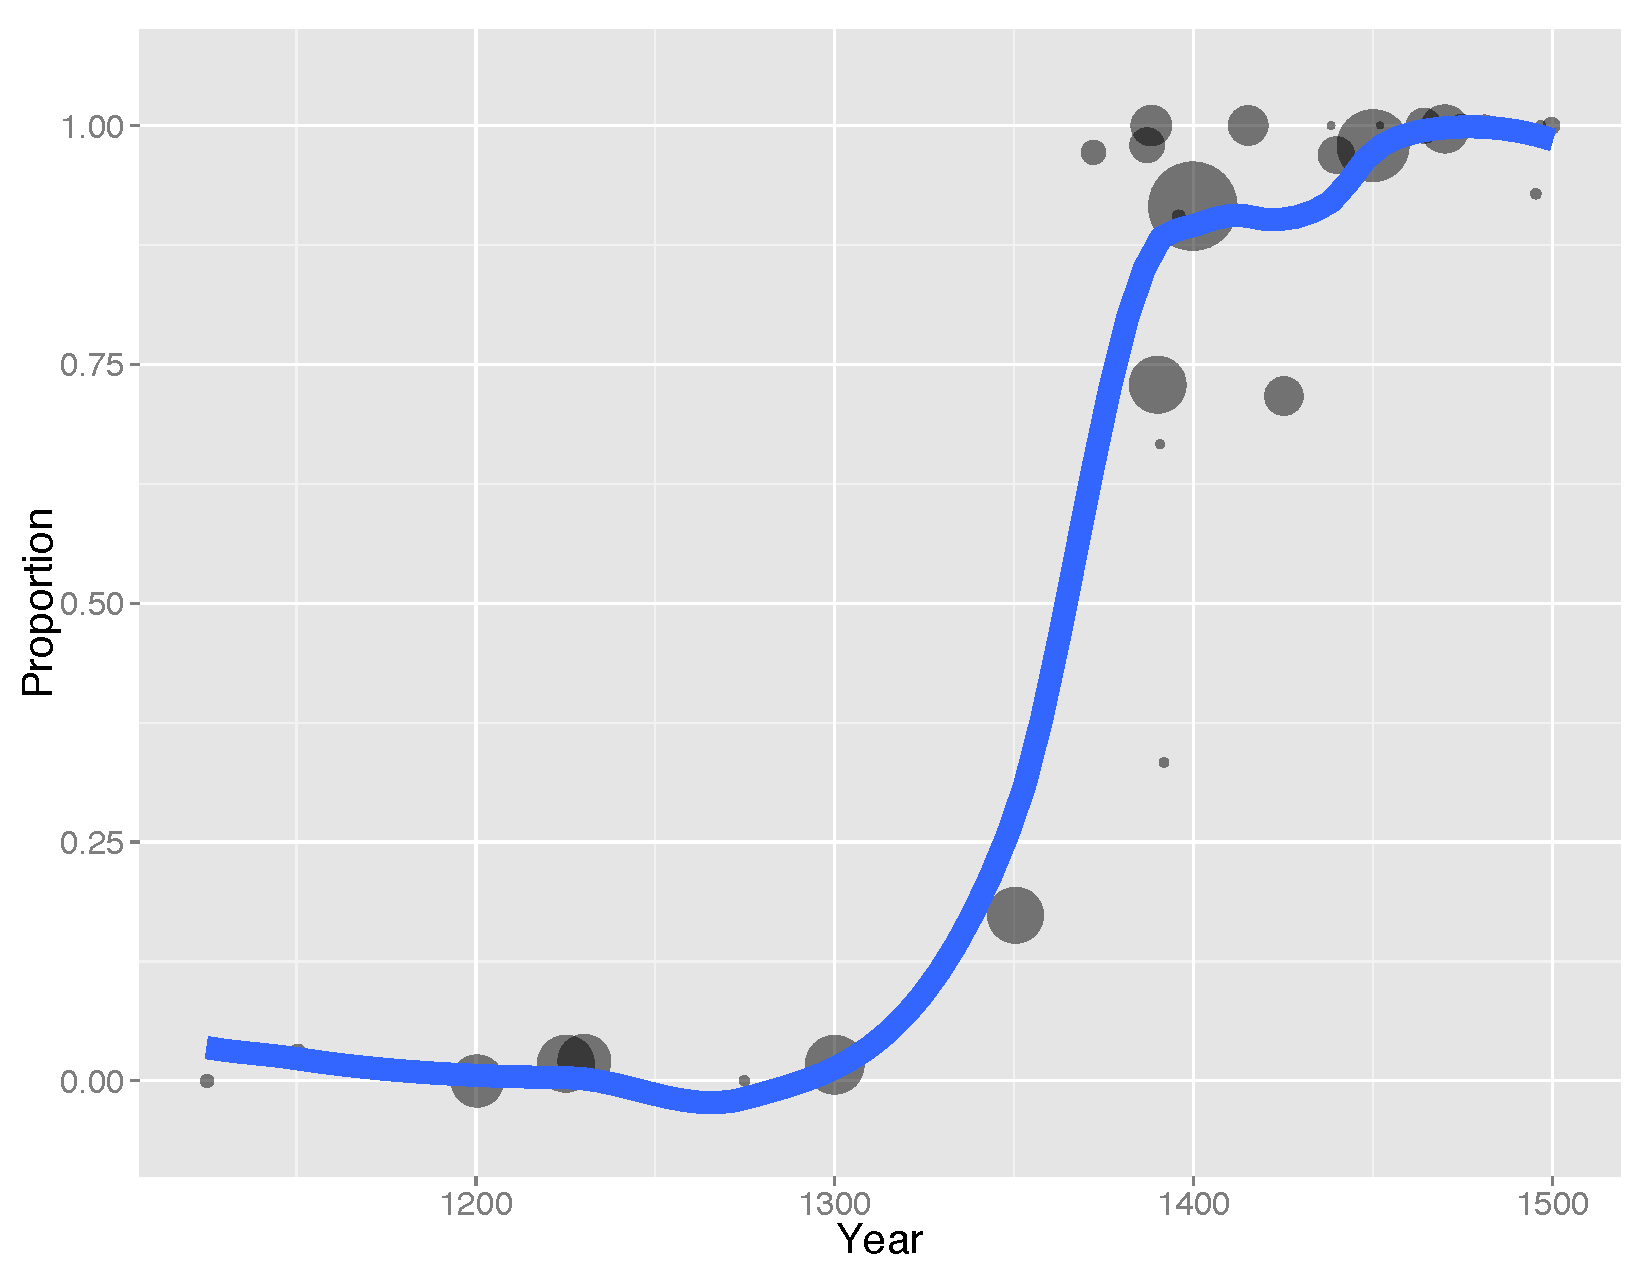
\includegraphics[width=.75\textwidth]{lump-plot2.pdf}}
%	\end{center}
%\end{frame}


\begin{frame}
\frametitle{A model of acquisition}

Given input from environment $L$, learner chooses grammar $G_i$ with probability $p_i$:
\begin{equation}
 \mbox{If $G_i \rightarrow s$ then }
\left\{
	\begin{array}{ll}
		p_i'  = p_i + \gamma (1-p_i)\\
		p_j'  = (1-\gamma)p_j &  \forall j \neq i
	\end{array}
\right.
\end{equation}

\begin{equation}
 \mbox{If $G_i \nrightarrow s$ then }
\left\{
	\begin{array}{ll}
		p_i'  = (1-\gamma ) p_i \\
		p_j'  = \frac{\gamma}{N - 1} + (1-\gamma)p_j & \forall j \neq i
	\end{array}
\right.
\end{equation}
	\vfill\hfill \parencite{yang2000internal}
\end{frame}


 \begin{frame}
 \frametitle{A model of acquisition}
 Linguistic environment $L$ is distribution over grammars:
     \begin{center}
         \begin{tikzpicture}
 	  \node (A) [draw,circle,minimum size=4cm]  at (0,0) {$\alpha_1$};
 	  \node (G1) [above of=A] {$G_1$};
 	  \node [draw,circle,minimum size=4cm] (B) at (0:3cm) {$\alpha_2$};
 	  \node (G2) [above of=B] {$G_2$};
 	\end{tikzpicture}         
     \end{center}
     	\vfill\hfill \parencite{yang2000internal}
 \end{frame}


\begin{frame}
\frametitle{A model of acquisition}
\begin{columns}[T] 
   \begin{column}{.5\textwidth}
   \begin{center}
	 \includegraphics[width=2.5in]{lrp-learning.png}
   \end{center}
   \end{column}
   \begin{column}{.5\textwidth}
   \begin{center}
	\includegraphics[width=2.5in]{lrp-dist.png}
    \end{center}
    \end{column}
  \end{columns}  
	\vfill \hfill \citep{narendra1989}
\end{frame}


\begin{frame}
\frametitle{The dynamics of acquisition}
\emph{Mean dynamics} of acquisition:
\begin{center}
	\only<1>{
	\begin{equation}
		\dot{p}_2 = p_2(1-p_2)\frac{\alpha_2 - \alpha_1}{p_1 \alpha_1 + p_2 \alpha_2}
	\end{equation}
	}
	\only<2->{
	\begin{equation}
		\dot{p} = p(1-p)\frac{s}{1- s(1-p)}
	\end{equation}
	\begin{equation}
		s =\frac{\alpha_2 - \alpha_1}{\alpha_2}
	\end{equation}
	\vfill \hfill (cf. \cite{ingason-etal2013})
	}
%%	\only<3>{
%	\begin{equation}
%		\dot{p} = p(1-p)s
%	\end{equation}
%	}
%	\only<3>{\hfill \footnotesize{(cf. \citealt{kroch1989,altmann-etal1983})}}
\end{center}	
\end{frame}


\begin{frame}
\frametitle{The dynamics of acquisition}
Simulations of population from same starting state with varying selection coefficient:
\begin{center}
 \includegraphics[width=.75\textwidth]{lrp-gain-eps-converted-to}\\
\end{center}

\end{frame}


\begin{frame}
\frametitle{The syntax of the formal cycle}
\begin{multicols}{3}
\small
        \Tree [.NegP [.XP $\varnothing$ ]
        [.Neg$'$ [.Neg \textcolor{red}{\emph{ne}}
        ] [.VP \edge[roof]; {...} ] ] ]

	 \Tree [.NegP [.XP \textcolor{blue}{\emph{not}} ]
        [.Neg$'$ [.Neg \textcolor{blue}{\emph{ne}}
        ] [.VP \edge[roof]; {...} ] ] ]

        \Tree [.NegP [.XP \textcolor{green}{\emph{not}} ]
        [.Neg$'$ [.Neg $\varnothing$ ]
        [.VP \edge[roof]; {...} ] ] ] 

\end{multicols}
\vfill \hfill \citep{frisch1997}
\end{frame}

\begin{frame}
\frametitle{The syntax of the formal cycle}
\only<3>{Acquisition dynamics \textbf{do not} predict transition from \textcolor{red}{\emph{ne}} to \textcolor{blue}{\emph{ne...not}}:}
\begin{center}
        \begin{tikzpicture}
	  \node (A) [draw,circle,minimum size=4cm]  at (0,0) {$\alpha_\varnothing$};
	  \node (G1) [above of=A] {\color{red} $G_\varnothing$};
	  \node [draw,circle,minimum size=4cm] (B) at (0:5cm) {$\alpha_{not}$};
	  \node (G2) [above of=B] {\color{blue} $G_{not}$};
	\end{tikzpicture}         
	
    \only<2->{ $s = \frac{\alpha_{not} - \alpha_\varnothing}{\alpha_{not}} = 0$}
    \end{center}
\end{frame}


\begin{frame}
\frametitle{The syntax of the formal cycle}
Acquisition dynamics \textbf{do not} predict transition from \textcolor{blue}{\emph{ne...not}} to \textcolor{green}{\emph{not}}:
\begin{center}
        \begin{tikzpicture}
	  \node (A) [draw,circle,minimum size=4cm]  at (0,0) {$\alpha_{ne}$};
	  \node (G1) [above of=A] {\color{blue} $G_{ne}$};
	  \node [draw,circle,minimum size=4cm] (B) at (0:5cm) {$\alpha_\varnothing$};
	  \node (G2) [above of=B] {\color{green} $G_\varnothing$};
	\end{tikzpicture}         
	
	 $s = 0$
    \end{center}

\end{frame}


\begin{frame}
\frametitle{The role of random drift}
\begin{columns}[T]  
   \begin{column}{.2\textwidth}
     % \begin{center}
  	  \vspace{12pt}
	  \includegraphics[height=1.2in]{bloomfield.jpg}   
     % \end{center}
   \end{column}
   \begin{column}{.8\textwidth}
      \begin{block}{}
      \begin{quote}
It may be urged that change in language is due ultimately to the deviations of individuals from the rigid system. But it appears that even here individual variations are ineffective; \textbf{whole groups} of speakers must, for some reason unknown to us, \textbf{coincide in a deviation}, if it is to result in a linguistic change
      \end{quote}
	\end{block}
    \end{column}
  \end{columns}
 \vfill\hfill \citep{bloomfield1927}
\end{frame}



\begin{frame}{The role of random drift}
%Imagine a finite population of frogs:
\begin{center}
 \includegraphics[width=2in]{red-frog.jpg} \hspace{1cm}  \includegraphics[width=2in]{blue-frog.jpg}
\end{center}
\end{frame}

\begin{frame}{The role of random drift}
\emph{Moran process}:
\begin{columns}[T] 
   \begin{column}{.5\textwidth}
   \begin{center}
	 \includegraphics[width=2in]{drift-selection.png}\\
	 \only<1>{?}
	  \only<2->{Drift ($s=0$, $N=100$)}
   \end{center}
   \end{column}
   \begin{column}{.5\textwidth}
   \begin{center}
	\includegraphics[width=2in]{selection-drift.png}\\
	\only<1-2>{?}
	 \only<3->{Selection ($s=0.1$, $N=100$)}
    \end{center}
    \end{column}
  \end{columns}  
  \vfill \hfill \citep{moran1958}
\end{frame}

\begin{frame}{The role of random drift}
\only<2>{\emph{Gaussian approximation to Moran process}:}
\begin{columns}[T] 
   \begin{column}{.5\textwidth}
   \begin{center}
	 \includegraphics[width=2in]{lump-plot1.pdf}\\
	\emph{\textcolor{red}{ne}} $\rightarrow$ \emph{\textcolor{blue}{(ne...)} \textcolor{mygreen}{not}} 
   \end{center}
   \end{column}
   \begin{column}{.5\textwidth}
   \begin{center}
	\includegraphics[width=2in]{lump-plot2.pdf}\\
	\emph{\textcolor{red}{ne} \textcolor{blue}{(...not)}} $\rightarrow$ \textcolor{mygreen}{not}
    \end{center}
    \end{column}
  \end{columns}  
    	\only<2>{\vfill\hfill  \citep{feder-etal2014}}
\end{frame}


%\begin{frame}
%\frametitle{The role of random drift}
%	\begin{center}
%		\only<1>{\textsc{\color{red} neg V neg} $\rightarrow$ \textsc{\color{blue} neg V neg} $\rightarrow$ \textsc{\color{green} V neg}}
%		\only<2>{\includegraphics[width=.75\textwidth]{neg-docs-lines.pdf}}
%		\only<3>{\includegraphics[width=.75\textwidth]{lump-plot1.pdf}}
%		\only<4>{\includegraphics[width=.75\textwidth]{lump-plot2.pdf}}
%	\end{center}
%\end{frame}



\begin{frame}{The role of random drift}
\emph{Fitness Increment Test}:
     \begin{table}[ht]
    %\begin{center}
    \begin{tabular}{@{}cp{3.5cm}p{3.5cm}@{}}
      \hline
        & \emph{\textcolor{red}{ne}} $\rightarrow$ \emph{\textcolor{blue}{(ne...)} \textcolor{mygreen}{not}} & \emph{\textcolor{red}{ne} \textcolor{blue}{(...not)}} $\rightarrow$ \textcolor{mygreen}{not}\\
      \hline
      $H_0$ & Drift ($\mu = 0$) \only<2->{$\xmark$} & Drift ($\mu = 0$) \only<4->{?} \\
      $H_1$ & Selection ($\mu > 0$) \only<2->{$\checkmark$}  & Selection ($\mu > 0$) \only<4->{?} \\
      \hline
		 & \only<2->{$ t(5) = 2.6394$}  & \only<4->{$t(5) = 1.7021$}\\
 		 & \only<2->{$ p = 0.0288$}  & \only<4->{$ p = 0.0820$}\\
      \hline
		 & \only<3->{$\hat{s} = 0.01913 $}  & \only<5->{$s=0$}\\
		 & \only<3->{$\hat{N} = 15900$}  & \only<5->{$\hat{N} = 506$}\\
      \hline
    \end{tabular}
    %\end{center}
  \end{table}
      	\vfill\hfill  (cf. \cite{feder-etal2014})
\end{frame}


\begin{frame}
  \frametitle{The role of random drift}
  Varying time for transition \textsc{\color{blue} neg V neg $\rightarrow$ \color{mygreen} V neg}:
  \begin{center}
    \begin{tikzpicture}[->,>=stealth',shorten >=1pt,auto,node distance=3cm]
      \draw[->] (0,0) -- (10,0);
      \node at (5,-1) {Time};
      \node[visible on=<2->] at (1,-.5) {Decades};
      \node[draw,align=center,visible on=<2->]  at (1,2) {English};
      \node[draw,align=center,visible on=<2->]  at (1,1) {High German};
      \node[visible on=<3->] at (6.75,-.5) {Centuries};
      \node[draw,align=center,visible on=<3->]  at (6.75,.75) {Low German};
      \node[draw,align=center,visible on=<3->]  at (6.75,1.5) {Dutch};      
      \node[draw,align=center,visible on=<3->]  at (6.75,2.25) {French};
      \node[visible on=<4->] at (9,-.5) {(Millenia?)};      
      \node[draw,align=center,visible on=<4->]  at (9,1.5) {Flemish};      
    \end{tikzpicture}
  \end{center}
  
\vfill \hfill \footnotesize{\citep{wallage2008,jager2008,breitbarth2009,martineau-mougeon2003,burridge1993,vanderAuwera-neuckermans2004,zeijlstra2004}}
\end{frame}

\begin{frame}
\frametitle{The formal cycle}
	\begin{center}
		\includegraphics[width=.75\textwidth]{neg-docs-lines.pdf}\\
		\emph{\textcolor{red}{ne}} $\rightarrow$ \emph{\textcolor{blue}{ne...not}} $\rightarrow$ \emph{\textcolor{mygreen}{not}}
	\end{center}
%	\vfill \hfill Data from PPCME \citep{ppcme2} 
\end{frame}



\section[]{}

\begin{frame}
\frametitle{The facts to be explained}
	\begin{center}
		\includegraphics[width=.75\textwidth]{neg-docs-lines.pdf}\\
		\emph{\textcolor{red}{ne}} $\rightarrow$ \emph{\textcolor{blue}{ne...not}} $\rightarrow$ \emph{\textcolor{mygreen}{not}}
	\end{center}
\end{frame}


\begin{frame}
  \frametitle{Language change}
  \begin{center}
    \begin{tikzpicture}[->,>=stealth',shorten >=1pt,auto,node distance=3cm]
      \node (A)      {Grammar $n$};
      \node (B) [below right of=A]  {Data $n$};
      \node (C) [above right of=B] {Grammar $n+1$};
      \node (D) [below right of=C] {Data $n+1$};
      \node (E) [above right of=D] {};
      \path[->] (A)  edge node[sloped, anchor=center, below] {\only<1>{Use} \only<2>{\textbf{Use}}} (B)
      (B) edge node[sloped, anchor=center, below] {Acquisition} (C)
      (C) edge[dashed] node {} (D)
      (D) edge[dashed] node {} (E);
    \end{tikzpicture}
  \end{center}
\end{frame}




\appendix

\section{Thanks}

\begin{frame}
\begin{center}
\huge Thank you!
\end{center}
\end{frame}

\begin{frame}
\frametitle{Thanks in particular to:}
\begin{center}
	\begin{itemize}
		\item Robin Clark, Mark Liberman, and Florian Schwarz
		\item Jon Stevens for ideas and discussions
		\item Aaron Ecay for PPCME queries, code, and discussion
		\item Josh Plotkin and Mitchell Johnson for code and discussion
		\item Penn graduate students and faculty
	\end{itemize}
\end{center}
\end{frame}

%\section{The functional cycle}

%\section{The formal cycle}
%
%\begin{frame}
%\frametitle{Dynamics of acquisition}
%Logistic curve versus acquisition dynamics:
%	\begin{center}
%		 \includegraphics[width=.75\textwidth]{lrp-log.png}\\
%	\end{center}
%	\vfill \hfill (cf. \citealt{kroch1989,altmann-etal1983})
%\end{frame}


\begin{frame}[allowframebreaks]{References}
\printbibliography
% \footnotesize{\printbibliography}
\end{frame}



\end{document}
